\documentclass{article}
\newcommand{\blind}{0}
% if you need to pass options to natbib, use, e.g.:
%\PassOptionsToPackage{numbers, compress}{natbib}
% before loading neurips_2021

\usepackage[authoryear]{natbib}
% ready for submission
\usepackage[preprint]{neurips_2021}

% to compile a preprint version, e.g., for submission to arXiv, add add the
% [preprint] option:
%     \usepackage[preprint]{neurips_2021}

% to compile a camera-ready version, add the [final] option, e.g.:
     %\usepackage[final]{neurips_2021}

% to avoid loading the natbib package, add option nonatbib:
%\usepackage[nonatbib]{neurips_2021}

\usepackage[utf8]{inputenc} % allow utf-8 input
\usepackage[T1]{fontenc}    % use 8-bit T1 fonts
\usepackage{hyperref}       % hyperlinks
\usepackage{url}            % simple URL typesetting
\usepackage{booktabs}       % professional-quality tables
\usepackage{amsfonts}       % blackboard math symbols
\usepackage{nicefrac}       % compact symbols for 1/2, etc.
\usepackage{microtype}      % microtypography
\usepackage{xcolor}         % colors
\usepackage{multirow}     

\usepackage{amsmath,amssymb,dsfont,color,bm,mathtools,enumitem}
\mathtoolsset{showonlyrefs}
\usepackage{amsthm}
\usepackage{subcaption}

\newtheorem{thm}{Theorem}
\newtheorem{lem}{Lemma}
\newtheorem{prop}{Proposition}
\newtheorem{pro}{Property}
\newtheorem{cor}{Corollary}
\usepackage{microtype}
\usepackage{wrapfig}

\usepackage{caption}

\DeclareCaptionFont{mysize}{\fontsize{9}{9.6}\selectfont}
\captionsetup{font=mysize}

\theoremstyle{definition}
\newtheorem{defn}{Definition}
\newtheorem{assumption}{Assumption}
\newtheorem{example}{Example}
\newtheorem{rmk}{Remark}

% If you use BibTeX in apalike style, activate the following line:
%\bibliographystyle{apalike}
\input macros.tex
\usepackage{mathrsfs}  
\def\caliB{\mathscr{B}}
\usepackage{float}

\setlength{\bibsep}{0.0pt}

\usepackage{xr}
\externaldocument{SCSG_smoothT_v2}


\setlength{\parskip}{0pt}


\begin{document}

\if1\blind
{   \title{Smooth tensor estimation with 
unknown permutations}
\author{%
  Chanwoo Lee \\
  University of Wisconsin-Madison\\
  \texttt{chanwoo.lee@wisc.edu} \\
  % examples of more authors
   \And
   Miaoyan Wang \\
   University of Wisconsin-Madison \\
   \texttt{miaoyan.wang@wisc.edu} }

    \maketitle
} \fi

\if0\blind
{
 \date{}
  \title{Appendix for ``Smooth tensor estimation with unknown permutations''}
\author{}
\maketitle
} \fi

\appendix
\vspace{-1.5cm}
The appendix includes extra numerical results and proofs to theorems.


\renewcommand{\thefigure}{S\arabic{figure}}
\setcounter{figure}{0}   
\renewcommand{\thetable}{S\arabic{table}}
\setcounter{table}{0}   

\section{Extra numerical results}

\subsection{Details in synthetic data experiment}\label{asec:sim}
{\bf Simulation models.} We describe the simulation set up in Section \ref{sec:sim} in details. We simulate order-3 $d$-dimensional tensors based on the permuted smooth tensor model~\eqref{eq:rep}. The symmetric tensors are generated based on functions $f$ in Table~\ref{tb:md}.

\begin{table}[htp]
    \centering
    \begin{tabular}{c|c|c|c}
        Model ID  &  $f(x,y,z)$ & CP rank & Tucker rank \\\hline
        1 &    $xyz$ & 1 & $(1,1,1)$\\
        2 &    $(x+y+z)/3$ & 3 & $(2,2,2)$\\
        3 & $(1+\exp(-3x^2+3y^2+3z^2))^{-1}$ &9& $(4,4,4)$ \\
        4 & $\log(1+\max(x,y,z))$ &$\geq 100$& $\geq (50,50,50)$ \\
        5 &  $\exp\left(-\max(x,y,z)-\sqrt{x}-\sqrt{y}-\sqrt{z}\right)$ &$\geq 100$& $\geq (50,50,50$)\\
    \end{tabular}
    \vspace{.5cm}
    \caption{Smooth functions in simulation. We define the numerical CP/Tucker rank as the minimal rank $r$ for which the relative approximation error is below $10^{-4}$. The reported rank in the table is estimated from a $100\times100\times100$  signal tensor generated by \eqref{eq:rep}.}
    \label{tb:md}
\end{table}

The generative functions involve compositions of operations such as polynomial, logarithm, exponential, square roots, etc. Notice that considered functions cover a reasonable range of model complexities from low rank to high rank. Two types of noise are considered: Gaussian noise and Bernoulli noise.
For the Gaussian model, we simulate continuous-valued tensors with i.i.d.\ noises drawn from $N(0,0.5^2)$. For the Bernoulli model, we generate binary tensors $\tY$ using the success probability tensor $\Theta \circ \pi$. The permutation $\pi$ is randomly chosen. For space consideration, only results for Models 1, 3, and 5 are presented in the paper. We first examine impacts of model complexity to estimation accuracy. We then compare Borda count estimation with alternative methods under a range of scenarios. 

 \begin{figure}[ht!]
    \centering
    \begin{subfigure}[b]{.9\textwidth}
    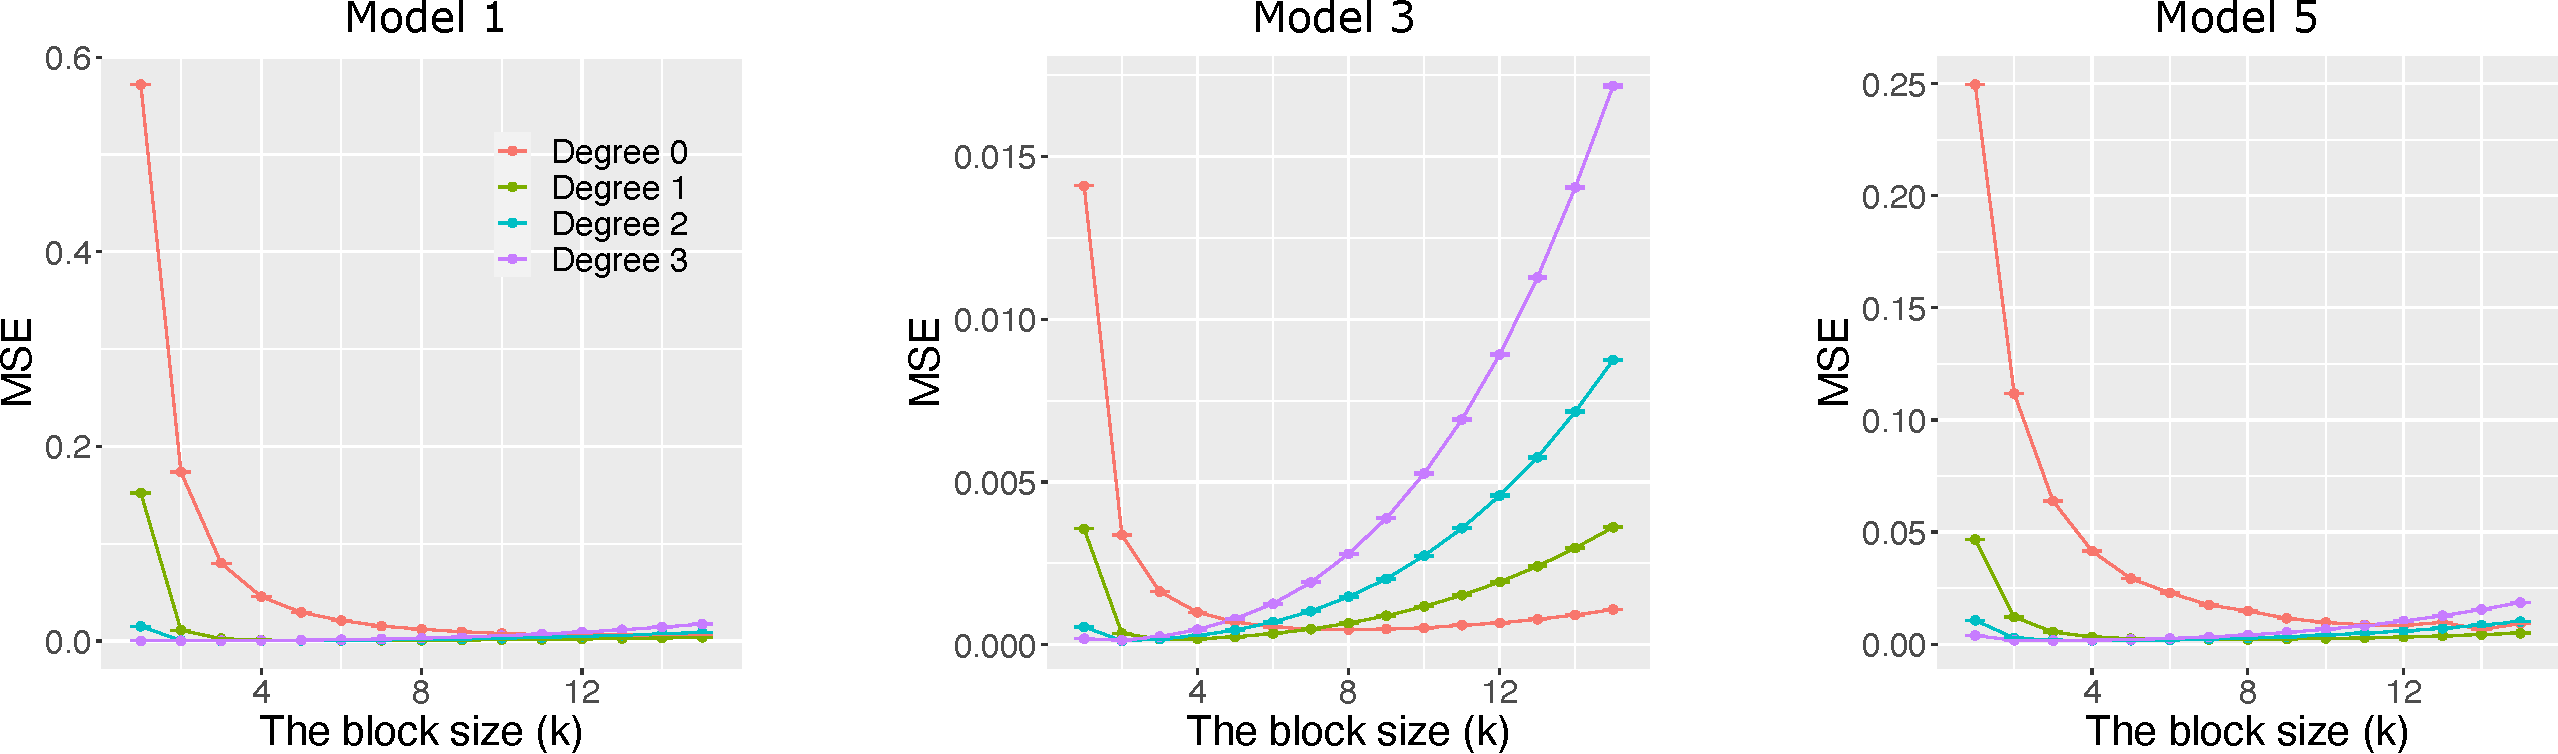
\includegraphics[width = \textwidth]{figures/deg_conti.pdf}    
    \end{subfigure}
    \vspace{.5cm}
    \begin{subfigure}[b]{.9\textwidth}
    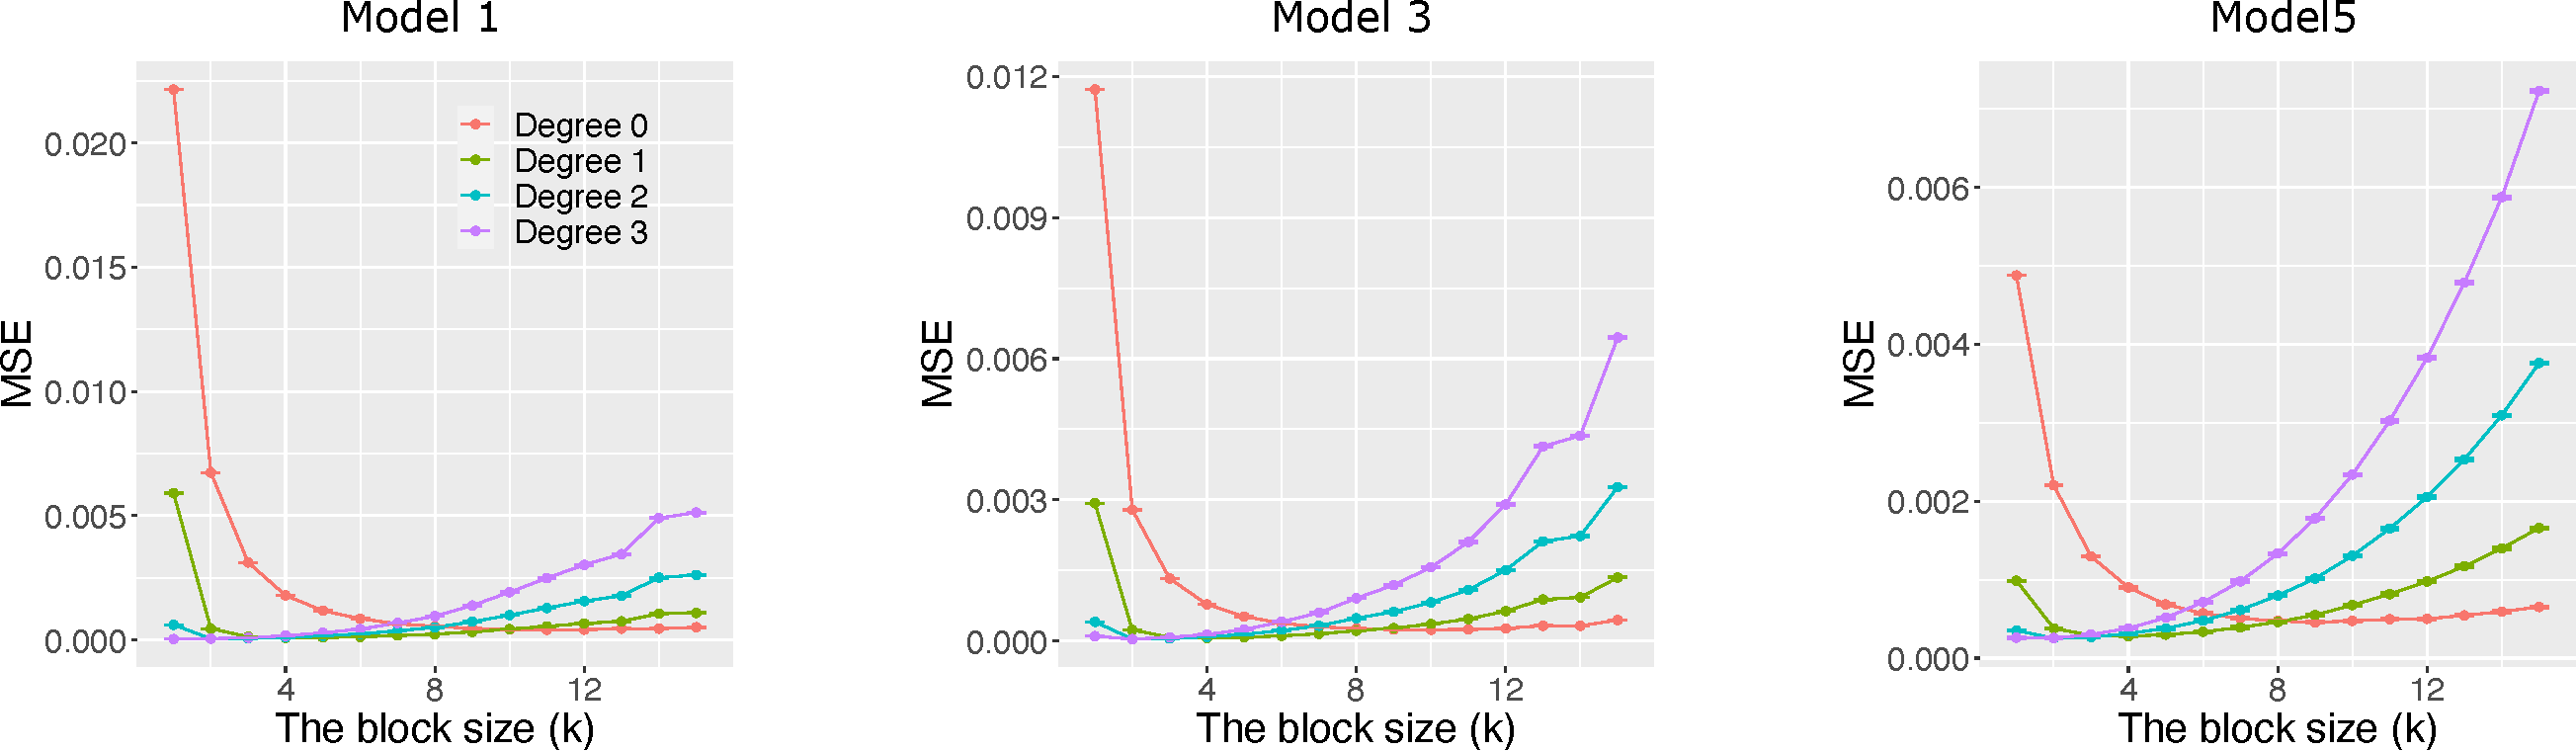
\includegraphics[width = \textwidth]{figures/deg_binary.pdf}    
    \end{subfigure}
    \caption{MSE versus the number of blocks based on different polynomial approximations. Columns 1-3 consider the Models 1, 3, and 5 respectively. Panel (a) is for continuous tensors, whereas (b) is for the binary tensors.}
    \label{fig:degk}
\end{figure}

\begin{figure}[ht!]
    \centering
    \begin{subfigure}[b]{\textwidth}
    \vspace{0.5cm}
    
    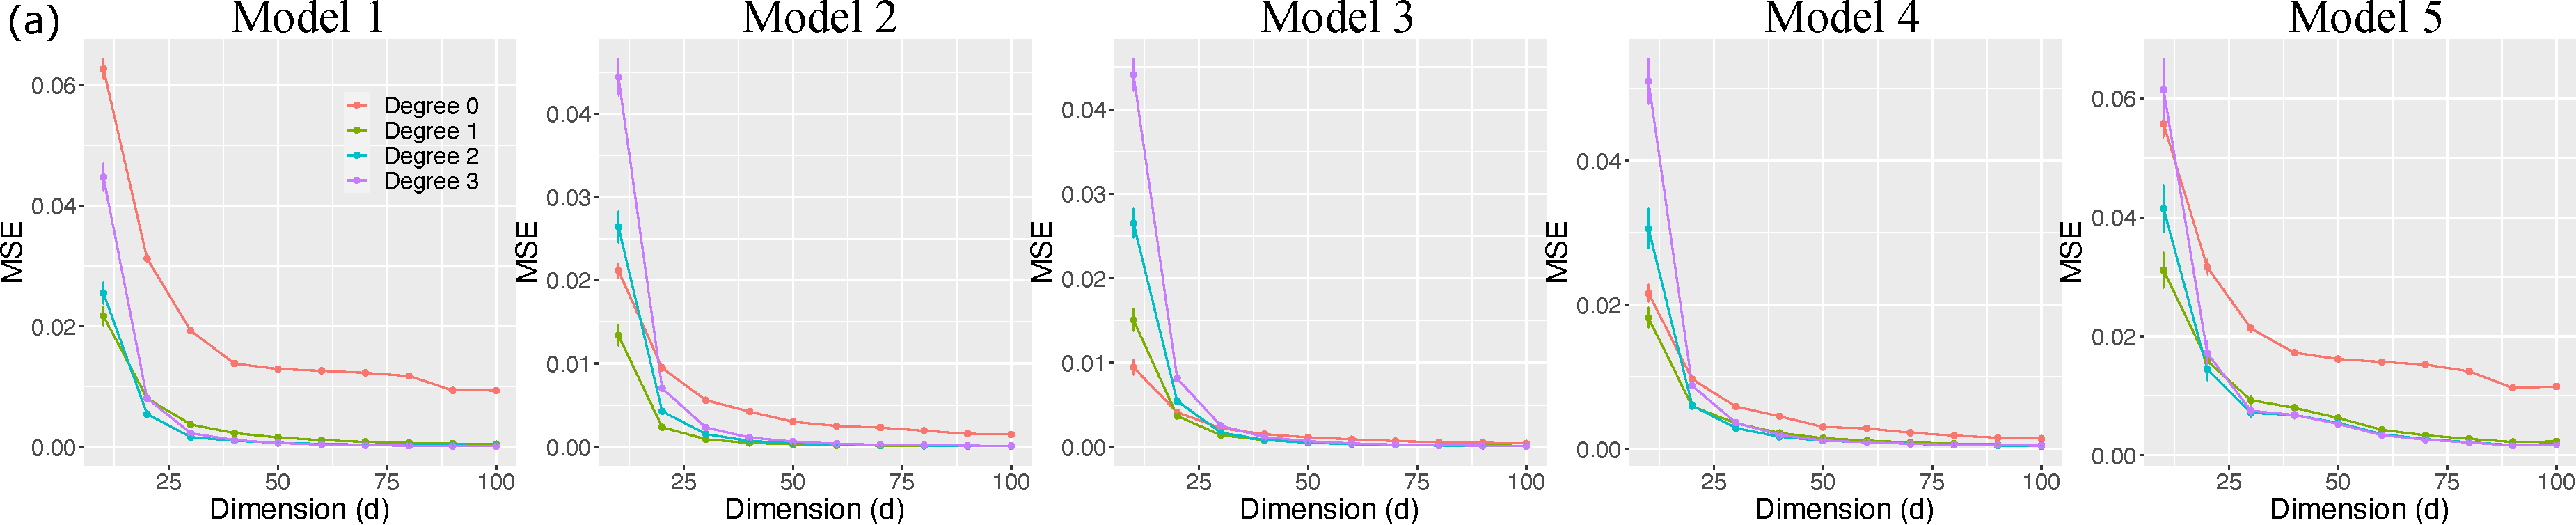
\includegraphics[width = \textwidth]{figures/deg_dim_c.pdf} 
    \vspace{0cm}
    \end{subfigure}
    \begin{subfigure}[b]{\textwidth}
    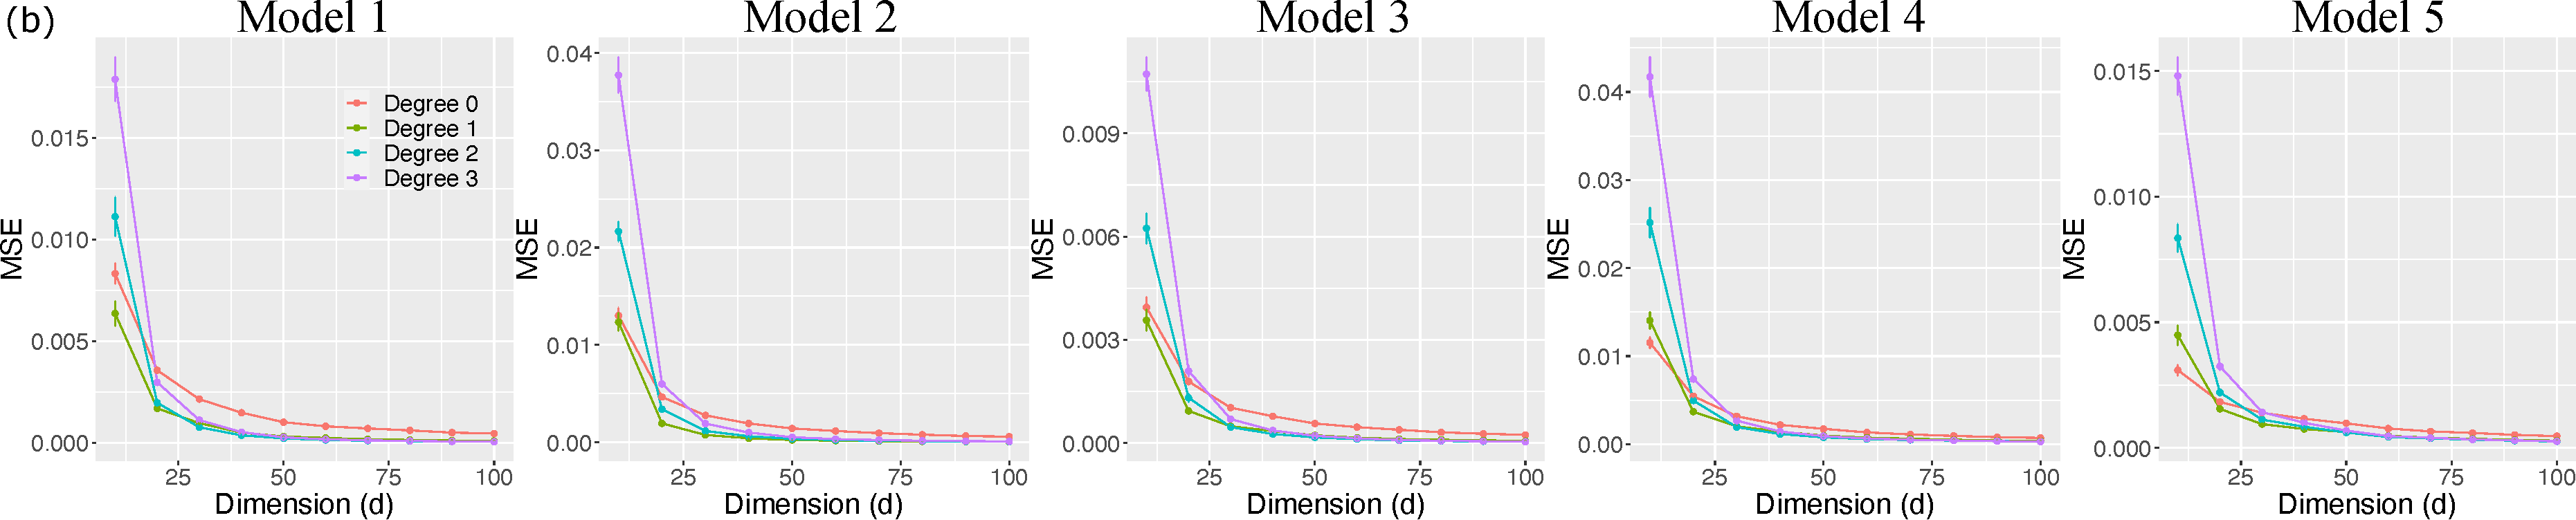
\includegraphics[width =\textwidth]{figures/deg_dim_b.pdf}    
    \end{subfigure}
    \caption{MSE versus the tensor dimension based on different polynomial approximations. Columns 1-5 consider the Models 1-5 in Table~\ref{tb:md} respectively. Panel (a) is for continuous tensors, whereas (b) is for the binary tensors.}
    \label{fig:degdim}
\end{figure}



\paragraph{Impacts of the number of blocks, tensor dimension, and polynomial degree.}
The first experiment examines the impact of the block number $k$ and degree of polynomial $\ell$ for the approximation. We fix the tensor dimension $d = 100$, and vary the number of blocks $k\in\{1,\ldots,15\}$ and polynomial degree $\ell\in\{0,1,2,3\}.$
Figure~\ref{fig:degk} demonstrates the trade-off in accuracy determined by the number of groups for each polynomial degree. The results confirm our bias-variance analysis in Theorem~\ref{thm:LSE}. While a large block number $k$ provides less biased approximation, this large $k$ renders the signal tensor estimation difficult within each block due to small sample size. In addition, we find that degree-2 polynomial approximation with the optimal $k$ gives the smallest MSE among all considered polynomial approximations. These observations are consistent with our theoretical results that the optimal number of blocks and polynomial degree are $(k^*,\ell^*)=(\tO(d^{3/7}),2)$. 

\begin{figure}[http!]
    \centering
    \begin{subfigure}[b]{.9\textwidth}
    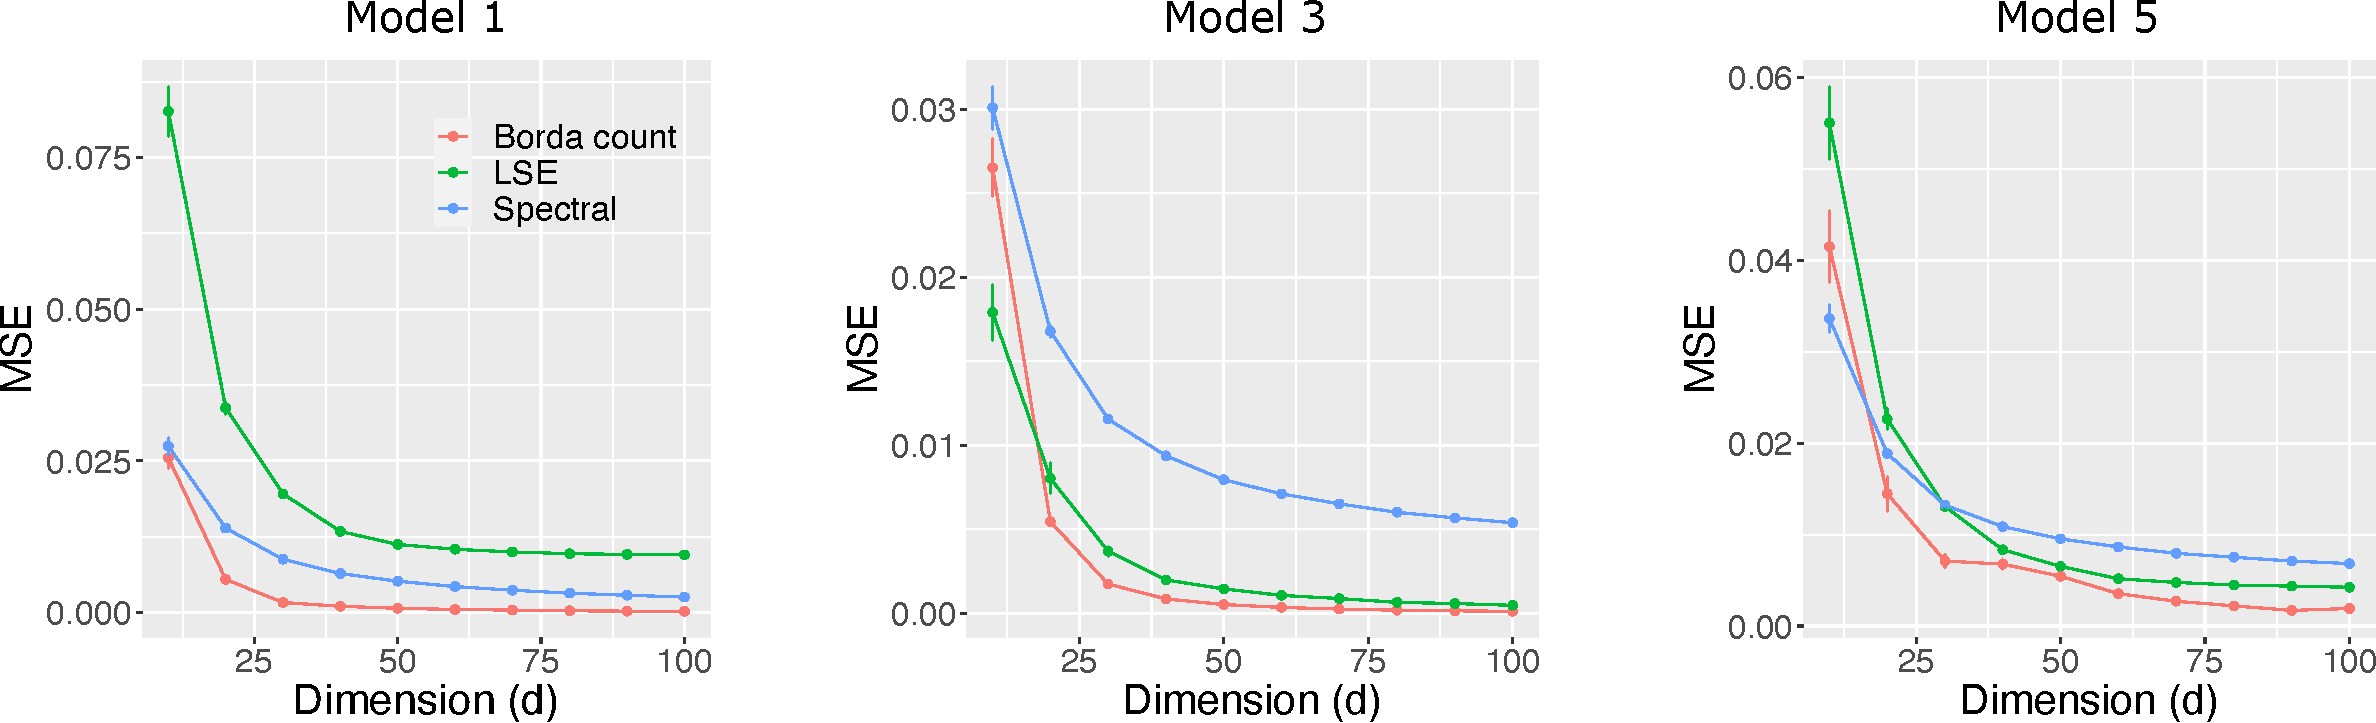
\includegraphics[width = \textwidth]{figures/altdim_conti.pdf}
       \vspace{.3cm}
    \end{subfigure}
    \begin{subfigure}[b]{.9\textwidth}
    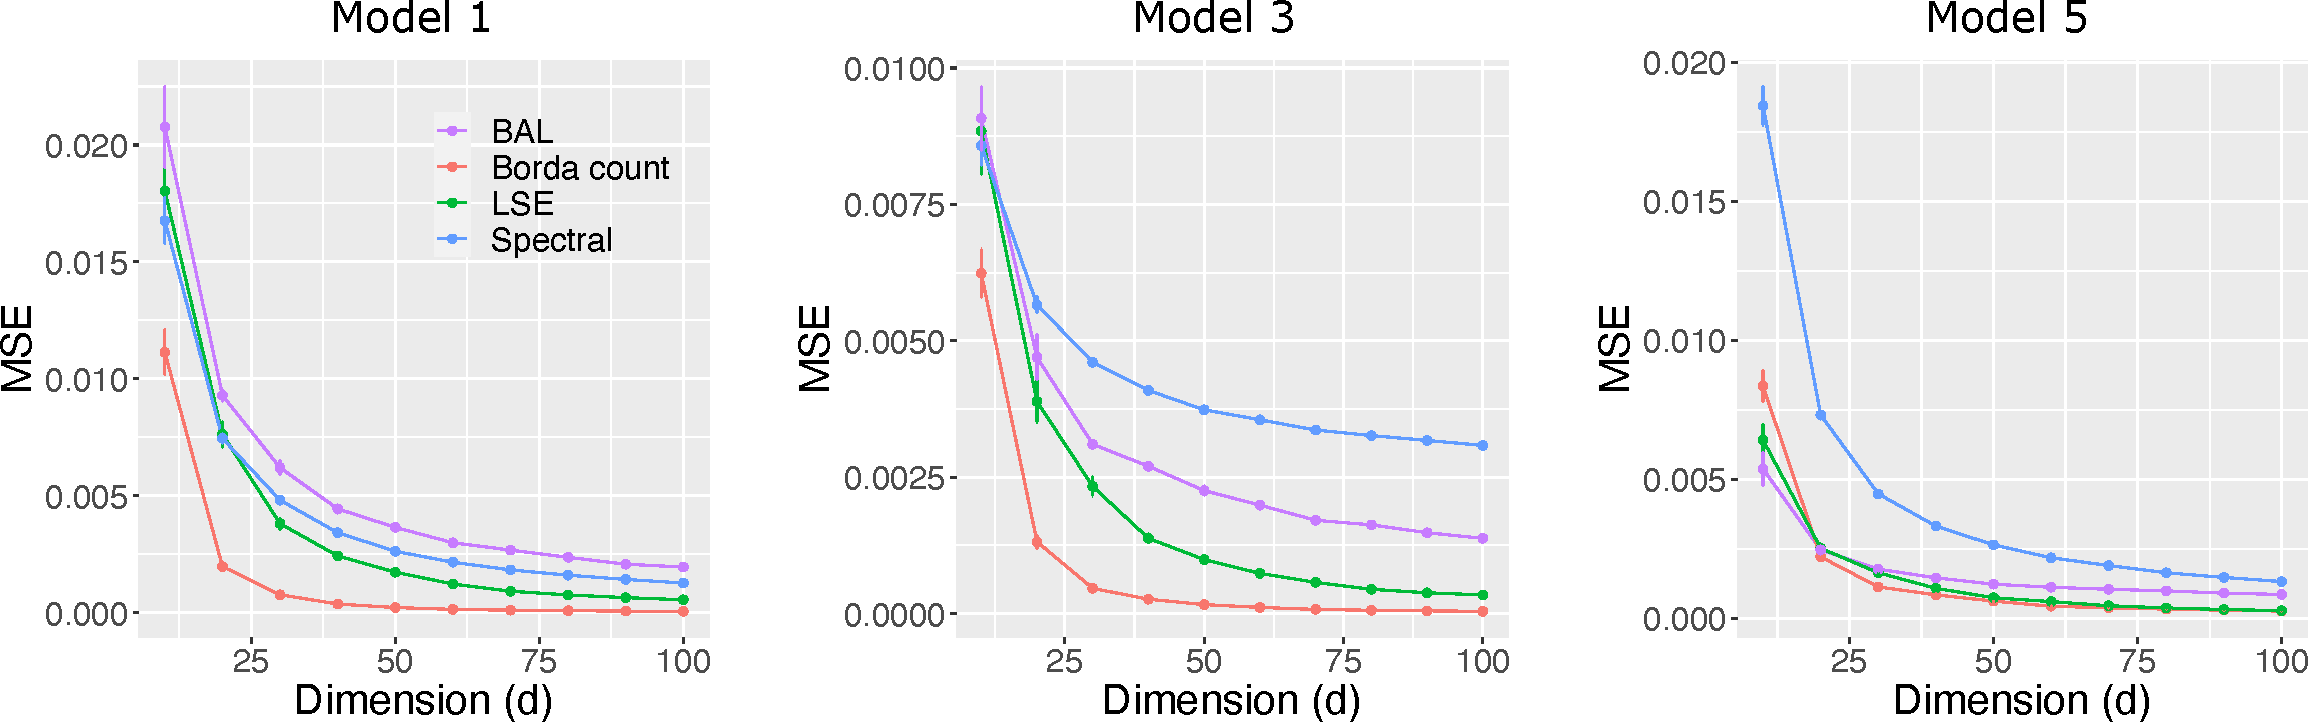
\includegraphics[width = \textwidth]{figures/altdim_binary.pdf}   
    \end{subfigure}
    \caption{MSE versus the tensor dimension based on different estimation methods. Columns 1-3 consider the Models 1, 3, and 5 in Table~\ref{tb:md} respectively. Panel (a) is for continuous tensors, whereas (b) is for the binary tensors.}
    \label{fig:method}
\end{figure}


The second experiment investigates the impact of the tensor dimension $d$ for various polynomial degrees. We vary the tensor dimension $d\in\{10,\ldots,100\}$ and polynomial degree $\ell\in\{0,1,2,3\}$ in each model configuration. We set optimal number of blocks as the one that gives the best accuracy. Figure~\ref{fig:degdim} compares the estimation errors among different polynomial approximations. The result verifies that the degree-2 polynomial approximation performs the best under the sufficient tensor dimension, which is consistent with our theoretical results. We emphasize that this phenomenon is different from the matrix case where the degree-0 polynomial approximation gives the best results~\citep{gao2021minimax,klopp2017oracle}.



\begin{figure}[ht!]
    \centering
    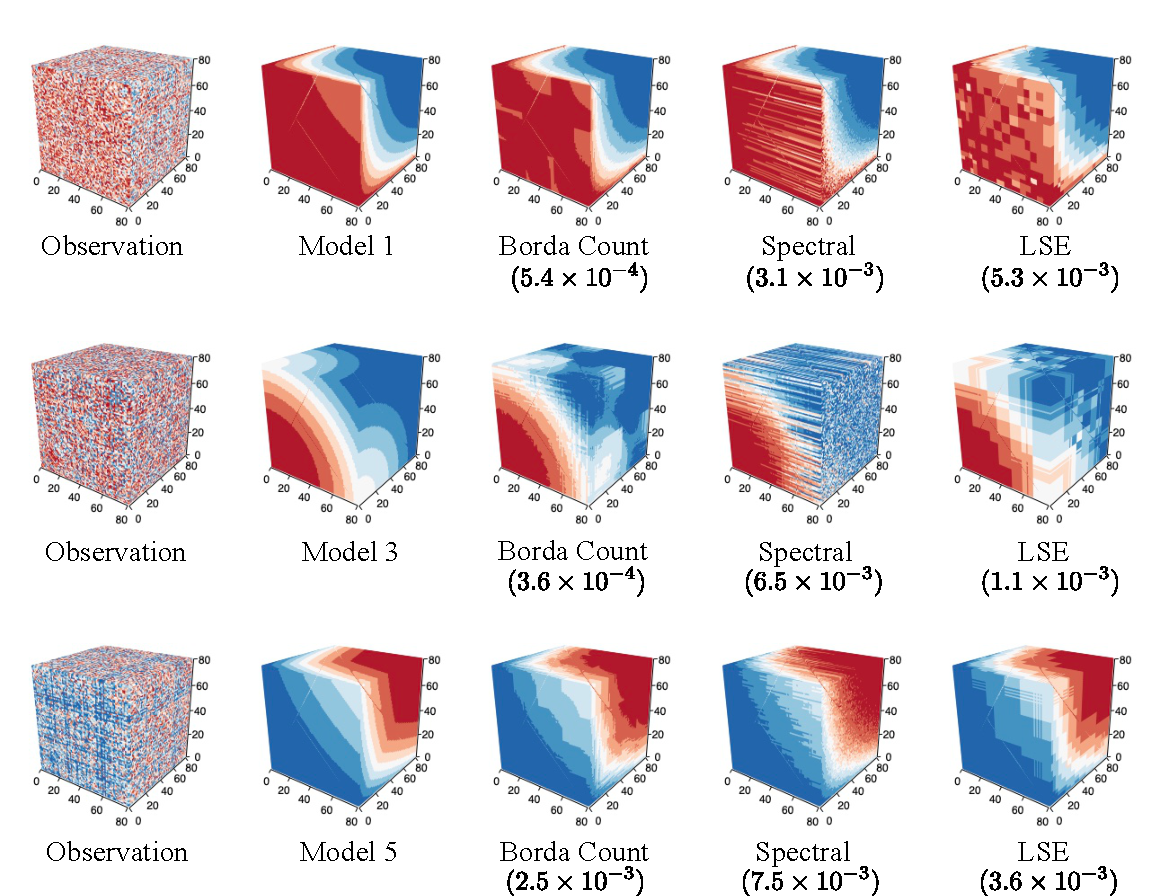
\includegraphics[width =0.9\textwidth]{figures/vfinal.pdf}
    \caption{Performance comparison among different methods. The observed data tensors, true signal tensors, and estimated signal tensors are plotted for Models 1, 3 and 5 in Table~\ref{tb:md} with fixed dimension $d = 80$. Numbers in parenthesis indicate the mean squared error.}
    \label{fig:contim}
\end{figure}


\paragraph{Comparison with alternative methods.} We compare our method ({\bf \small Borda Count}) with several popular alternative methods. 
\begin{itemize}[wide, labelwidth=0pt, labelindent=0pt,itemsep=0ex]
    \item  Spectral method ({\bf \small Spectral})~\citep{xu2018rates} that performs universal singular value thresholding~\citep{chatterjee2015matrix} on the unfolded tensor.
    \item Least-squares estimation ({\bf \small LSE}) \citep{gao2021minimax} which solves the optimization problem \eqref{eq:lseopt} with constant block approximation ($\ell=0$) based on spectral $k$-means. We extend the matrix-based biclustering algorithm to higher-order tensors~\citep{han2020exact}. 
    \item Least-squares estimation ({\bf \small BAL}) \citep{balasubramanian2021nonparametric} which solves the optimization problem \eqref{eq:lseopt} with constant block approximation ($\ell=0$). This tensor-based algorithm is only available for binary observations because it uses count-based statistics. Therefore, we only use this algorithm for the Bernoulli model.
\end{itemize}


We choose degree-2 polynomial approximation as our theorems suggested, and vary tensor dimension $d\in\{10,\ldots,100\}$ under each model configuration. For {\bf \small Borda Count} and {\bf \small LSE}, we choose the block numbers that achieve the best performance in the corresponding outputs. For {\bf \small Spectral} method, we set the hyperparameter (singular-value threshold) that gives the best performance. 


Figure~\ref{fig:method} shows that our algorithm {\bf \small Borda Count} achieves the best performance in all scenarios as the tensor dimension increases. The poor performance of {\bf \small Spectral} can be explained by the loss of multilinear structure in the tensor unfolding procedure. The sub-optimality of {\bf \small LSE} is possibly due to its limits in both statistics and computations. Statistically, our theorems have shown that constant block approximation results in sub-optimal rates compared to polynomial approximation. Computationally, the least-squares optimization~\eqref{eq:lseopt} is highly non-convex and computationally unstable. 
Figure~\ref{fig:contim} displays true signal tensors of three models and corresponding observed tensors of dimension $d = 80$ with Gaussian noise. We use oracle permutation $\pi$ to obtain the estimated signal tensor from the estimated permuted signal tensor $\hat\Theta\circ\hat\pi$ for the better visualization and comparisons. As shown in the figure, we see clearly that our method achieves the best signal recovery, thereby supporting the numerical results in Figure~\ref{fig:method}.
The outperformance of {\bf \small Borda count} demonstrates the efficacy of our method.


\paragraph{Investigation of non-symmetric tensors.}
Our models and techniques easily extend to non-symmetric tensors. We use non-symmetric functions to generate order-3 signal tensors. based on functions in Table~\ref{tb:md2}. 
\begin{table}[ht]
    \centering
    \begin{tabular}{c|c}
        Model ID  &  $f(x,y,z)$  \\\hline
        1 &    $xy+z$ \\
        2&  $x^2+y +yz^2$\\
        3 & $x(1+\exp(-3(x^2+y^2+z^2)))^{-1}$\\
        4 & $\log(1+\max(x,y,z)+x^2+yz)$ \\
        5 &  $\exp\left(-x-\sqrt{y}-z^3\right)$
    \end{tabular}
        \vspace{.2cm}
    \caption{List of non-symmetric smooth functions in simulation.}
    \label{tb:md2}
\end{table}


We fix the tensor dimension ${30\times40\times 50}$ and assume that the noise tensors are from Gaussian distribution. Similar to other simulations, we evaluate the accuracy of the estimation by MSE and report the summary statistics across $n_{\text{sim}} = 20$ replicates. The hyperparameters are chosen via cross-validation that give the best accuracy for each method. Table~\ref{tb:hyper} summarizes the choice of hyperparameters. Table~\ref{tb:asymresult} compares the MSEs from repeated simulations based on different methods under Models 1-5. We find that Borda count estimation outperforms all alternative methods for non-symmetric tensors. The results demonstrate the applicability of our method to general tensors. 


\begin{table}[ht!]
\centering
    \begin{tabular}{c|c|c|c|c|c}
        Method &  Model 1 & Model 2 & Model 3& Model 4 & Model 5  \\\hline
        Borda count &   (2,1,2)&(1,2,2)& (1,3,3) &(2,1,2)&(1,4,4)\\
        LSE &(6,2,3)&(8,5,8)&(6,9,6)&(9,5,6)&(7,9,3)\\
        Spectral & (1,24)&(3,48)&(1,48)&(1,28)&(1,22)\\
    \end{tabular}
    \vspace{.2cm}
    \caption{Hyperparameters for the methods under Models 1-5 in Table~\ref{tb:md2}. For {\bf \small Borda count} and {\bf \small LSE} methods, the values in the table indicate the number of blocks. For {\bf \small Spectral} method, the first value indicates the tensor unfolding mode, while the second one represents the singular value threshold.}
    \label{tb:hyper}
\end{table}


\begin{table}[h!]
    \centering
    \begin{tabular}{c|c|c|c|c|c}
        Method &  Model 1 & Model 2 & Model 3& Model 4 & Model 5  \\\hline
        Borda count &  {\bf 0.57 (0.01)}&{\bf 0.51 (0.02)}& {\bf0.87 (0.02)} &{\bf1.02 (0.02)}& {\bf2.56 (0.21)}\\
        LSE &23.58 (0.03)&7.70 (0.04)&9.45 (0.05)&3.29 (0.05)&9.93 (0.03)\\
        Spectral & 10.76 (0.06)&10.64 (0.05)&6.27 (0.05)&10.90 (0.06)&5.24 (0.04)
    \end{tabular}
        \vspace{.2cm}
    \caption{MSEs from 20 repeated simulations based on different methods. All numbers are displayed on the scales $10^{-3}$. Standard errors are reported in parenthesis.}
    \label{tb:asymresult}
\end{table}




\subsection{Details on Chicago crime data analysis}\label{subsec:chicago}

\begin{table}[h!]
\centering
    \begin{tabular}{c|c|c}
         &  Constant block model & Permuted smooth tensor model \\\hline
    
        MSE &   0.399 (0.009) &  0.283 (0.006)\\
        Block number &    $(7,11,10)$  & $(6,4,10)$
    \end{tabular}
        \vspace{.2cm}
    \caption{Performance comparison in Chicago data analysis. Reported MSEs are averaged
over five runs of cross-validation, with 20\% entries for testing and 80\% for training, with standard
errors in parentheses. Block number is set to achieve the best prediction performance.}\label{tab:MSE}
\end{table}

We compare the prediction performance based on constant block model and our permuted smooth tensor model. Notice that constant block model uses $\ell=0$ approximation, whereas our permuted smooth tensor model uses $\ell=2$ approximation. Table~\ref{tab:MSE} shows the mean squared error over five runs of cross-validation, with 20\% entries for testing and 80\% for training. We find that the permuted smooth tensor model substantially outperforms the classical constant block models. We emphasize that our method does not necessarily assume the block structure. The comparison supports our premises that permuted smooth tensor model with polynomial approximation performs better than common constant block models in this application. 

We also investigate the ten groups of crime types clustered by our method. Table~\ref{tb:crimetb} shows that the clustering captures the similar type of crimes. For example, group 2 consists of misdemeanors such as public indecency, non-criminal, and concealed carry license violation, while group 6 represents sex-related offenses such as prostitution, sex offense, and crime sexual assault.

\begin{table}[h!]
\centering
    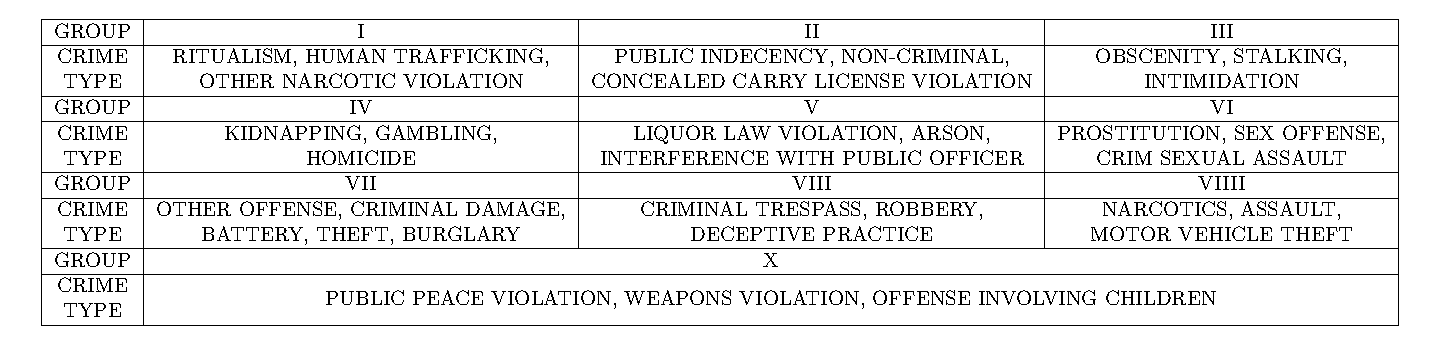
\includegraphics[width = \textwidth]{figures/crimetable.pdf}
    \caption{Groups of crime types learned based on the Borda count estimation.}
    \label{tb:crimetb}
\end{table}

\section{Proofs}



\subsection{Proof of Theorem~\ref{thm:LSE}}\label{sec:proofLSE}

Smoothness of the function $f$ in \eqref{eq:rep} plays an important role in the block-wise polynomial approximation. The following lemma explains the role of smoothness in the approximation. 

\begin{lem}[Block-wise polynomial tensor approximation]\label{lem:approx}
Suppose  $\Theta\in\tP(\alpha,L)$. Then, for every block number $k\leq d$, and degree $\ell\in \bbN_{\geq 0}$, we have the approximation error
\begin{align}
   \inf_{\tB\in\caliB(k,\ell)} \frac{1}{d^m}\FnormSize{}{\Theta-\tB}^2\lesssim \frac{L^2}{k^{2\min(\alpha,\ell+1)}}.
\end{align}
\end{lem}
Lemma~\ref{lem:approx} implies that we can always find a block-wise polynomial tensor close to the signal tensor generated from $\alpha$-H\"older smooth function $f$. The approximation error decays with block number $k$ and degree $\min(\alpha,\ell+1)$. 
\begin{proof}[Proof of Lemma~\ref{lem:approx}]
Recall that we denote $\tE_k$ as the $m$-way partition
\begin{align}
    \tE_k = \{\bigtimes_{a=1}^m z^{-1}(j_a)\colon (j_1,\ldots,j_m)\in [k]^m\}, 
\end{align}
where $z\colon [d]\rightarrow[k]$ is the canonical clustering function such that $z(i) = \lceil ki/d\rceil,$ for all $i \in[d]$, and we use the shorthand $\bigtimes_{a=1}^m$ to denote the Cartesian product of $m$ sets. For a given partition  $ \bigtimes_{a=1}^m z^{-1}(j_a)\in\tE_k$, fix any index  $(i_1^0,\ldots,i_m^0)\in \bigtimes_{a=1}^m z^{-1}(j_a)$. Then, we have 
\begin{align}\label{eq:ind}
\|(i_1,\ldots,i_m)-(i_1^0,\ldots,i_m^0)\|_\infty \leq \frac{d}{k},
\end{align} 
for all $(i_1,\ldots,i_m)\in \bigtimes_{a=1}^m z^{-1}(j_a)$.
We define the block-wise degree-$\ell$ polynomial tensor $\tB$ based on the partition $\tE_k$ as
\begin{align}
    \tB(i_1,\ldots,i_m) = \text{Poly}^{j_1,\ldots,j_m}_{\min(\lfloor \alpha \rfloor,\ell)}\left(\frac{i_1-i_1^0}{d},\ldots\frac{i_m-i_m^0}{d}\right), \quad \text{for all } (i_1,\ldots,i_m)\in \bigtimes_{a=1}^m z^{-1}(j_a),
\end{align}
where $\text{Poly}^{j_1,\ldots,j_m}_{\min(\lfloor \alpha \rfloor,\ell)}$ denotes a degree-$\ell$ polynomial function satisfying
\begin{align}\label{eq:polyapp}
\left|f\left(\frac{i_1}{d},\ldots,\frac{i_m}{d}\right)-\text{Poly}^{j_1,\ldots,j_m}_{\min(\lfloor \alpha \rfloor,\ell)}\left(\frac{i_1-i_1^0}{d},\ldots\frac{i_m-i_m^0}{d}\right)\right|\leq L\left\|\left(\frac{i_1-i_1^0}{d},\ldots,\frac{i_m-i_m^0}{d}\right)\right\|_\infty^{\min(\alpha,\ell+1)},
\end{align}
for all $(i_1,\ldots,i_m)\in \bigtimes_{a=1}^m z^{-1}(j_a).$
Notice that we can always find such polynomial function by $\alpha$-H\"older smoothness of the generative function $f$.
Based on the construction of block-wise degree-$\ell$ polynomial tensor $\tB$, we have 
\begin{align}
   & \frac{1}{d^m}\FnormSize{}{\Theta-\tB}^2\\
=&\ \frac{1}{d^m} \sum_{(i_1,\ldots,i_m)\in[d]^m}|\Theta(i_1,\ldots,i_m)-\tB(i_1,\ldots,i_m)|^2\\
=&\ \frac{1}{d^m}\sum_{(j_1,\ldots,j_m)\in[k]^m}\sum_{(i_1,\ldots,i_m)\in \bigtimes_{a=1}^m z^{-1}(j_a)}\bigg|f\left(\frac{i_1}{d},\ldots,\frac{i_m}{d}\right)-\text{Poly}^{j_1,\ldots,j_m}_{\min(\lfloor \alpha \rfloor,\ell)}\left(\frac{i_1-i_1^0}{d},\ldots,\frac{i_m-i_m^0}{d}\right)\bigg|^2\\
    \lesssim &\ \frac{L^2}{d^m}\sum_{(j_1,\ldots,j_m)\in[k]^m}\sum_{(i_1,\ldots,i_m)\in \bigtimes_{a=1}^m z^{-1}(j_a)} \left\|\left(\frac{i_1-i_1^0}{d},\ldots,\frac{i_m-i_m^0}{d}\right)\right\|_\infty^{2\min(\alpha,\ell+1)}\\
    \leq&\ \frac{L^2}{k^{2\min(\alpha,\ell+1)}},
\end{align}
where the first inequality uses~\eqref{eq:polyapp} and the second inequality is from \eqref{eq:ind}.
\end{proof}



\begin{proof}[Proof of Theorem~\ref{thm:LSE}] By Lemma~\ref{lem:approx}, there exists a block-wise polynomial tensor $\tB\in\caliB(k,\ell)$ such that
\begin{equation}\label{eq:approx}
\FnormSize{}{\tB-\Theta}^2\lesssim {L^2d^m\over k^{2\min(\alpha,\ell)}}.
\end{equation}
By the triangle inequality,
\begin{equation}\label{eq:tri}
\FnormSize{}{\hat\Theta^\textup{LSE}\circ\hat\pi^\textup{LSE} -\Theta\circ \pi}^2\leq 2\FnormSize{}{\hat\Theta^\textup{LSE}\circ\hat\pi^\textup{LSE} -\tB\circ \pi}^2+2\underbrace{\FnormSize{}{\tB\circ \pi-\Theta\circ \pi}^2}_{\textup{Lemma~\ref{lem:approx}}}.
\end{equation}
Therefore, it suffices to bound $\FnormSize{}{\hat\Theta^\textup{LSE}\circ\hat\pi^\textup{LSE} -\tB\circ \pi}^2$. By the global optimality of least-square estimator, we have
\begin{align}
\FnormSize{}{\hat\Theta^\textup{LSE}\circ\hat\pi^\textup{LSE} -\tB\circ \pi}&\leq \left\langle {\hat \Theta^\textup{LSE}\circ \hat \pi^\textup{LSE}-\tB\circ \pi \over \FnormSize{}{ \hat \Theta^\textup{LSE}\circ \hat \pi^\textup{LSE}-\tB\circ \pi}},\ \tE+(\Theta\circ \pi-\tB\circ \pi) \right \rangle \\
&\leq \sup_{\pi, \pi'\colon[d]\to[d]}\sup_{\tB, \tB'\in \caliB(k,\ell)} \left\langle {\tB'\circ \pi'-\tB\circ \pi \over \FnormSize{}{\tB'\circ \pi'-\tB\circ \pi}}, \tE \right \rangle+\underbrace{\FnormSize{}{\tB\circ \pi-\Theta\circ \pi}}_{\textup{Lemma~\ref{lem:approx}}}.
\end{align}
Now we bound inner product term. For fixed $\pi,\pi'$, let $\mP$ and $\mP'$ be permutation matrices corresponding to permutations $\pi$ and $\pi'$ respectively. 
We express vectorized block-wise degree-$\ell$ polynomial tensors, $\text{vec}(\tB)$ and $\text{vec}(\tB')$, by discrete polynomial functions. Specifically, denote $\text{vec}(\tB)=\mX\mbeta$ and $\text{vec}(\tB')=\mX\mbeta'$, where $\mX\in\bbR^{d^m\times k^m(k+m)^\ell}$ is a design matrix consisting of $m$-multivaraite degree-$\ell$ polynomial basis over grid design $(1/d,\ldots,d/d)$, $\mbeta$ and $\mbeta'\in\bbR^{k^m(k+m)^\ell}$ are corresponding coefficient vectors. Notice that the number of coefficients for $m$-multivariate polynomial of degree-$\ell$ is $\ell+m \choose \ell$. We choose to use $(k+m)^\ell$ coefficients for each block for notational simplicity. Therefore, we rewrite the inner product
\begin{align}
   \left\langle {\tB'\circ \pi'-\tB\circ \pi \over \FnormSize{}{\tB'\circ \pi'-\tB\circ \pi}}, \tE \right \rangle &=  \left\langle {(\mP')^{\otimes m}\text{vec}(\tB')-(\mP)^{\otimes m}\text{vec}(\tB) \over \FnormSize{}{(\mP')^{\otimes m}\text{vec}(\tB')-(\mP)^{\otimes m}\text{vec}(\tB)}}, \tE \right \rangle\\
    &=\left\langle {(\mP')^{\otimes m}\mX\mbeta'-(\mP)^{\otimes m}\mX\mbeta \over \FnormSize{}{(\mP')^{\otimes m}\mX\mbeta'-(\mP)^{\otimes m}\mX\mbeta}}, \tE \right \rangle\\&=
     \left\langle {\mA\mc \over \FnormSize{}{\mA\mc}}, \tE \right \rangle,
\end{align}
where we define $\mA := \begin{pmatrix}\mP' &-\mP\end{pmatrix}\begin{pmatrix}\mX & 0\\ 0&\mX\end{pmatrix}\in\bbR^{d^m\times 2k^m(k+m)^\ell}$ and $\mc:=\begin{pmatrix} \mbeta'\\\mbeta\end{pmatrix}\in\bbR^{2k^m(k+m)^\ell}.$
By Lemma~\ref{lem:embedding}, we have 
\begin{align}\label{eq:embedding}
\sup_{\tB, \tB'\in \caliB(k,\ell)} \left\langle {\tB'\circ \pi'-\tB\circ \pi \over \FnormSize{}{\tB'\circ \pi'-\tB\circ \pi}}, \tE \right \rangle \leq \sup_{\mc\in \bbR^{2k^m(\ell+m)^\ell } }\left\langle {\mc\over \vnormSize{}{\mc}},\ e \right\rangle,
\end{align}
where  $e\in\bbR^{2k^m(k+m)^\ell}$ is a vector consisting of i.i.d.\ sub-Gaussian entries with variance proxy $\sigma^2$. 
By the union bound of Gaussian maxima over countable set $\{\pi,\pi'\colon [d]\to[d]\}$, we obtain
\begin{align}\label{eq:union}
    \mathbb{P}&\left(\sup_{\pi, \pi'\colon[d]\to[d]}\sup_{\tB, \tB'\in \caliB(k,\ell)} \left\langle {\tB'\circ \pi'-\tB\circ \pi \over \FnormSize{}{\tB'\circ \pi'-\tB\circ \pi}}, \tE \right \rangle\geq t\right)\\
    &\leq \sum_{\pi,\pi'\in[d]^d}\mathbb{P}\left(\sup_{\tB, \tB'\in \caliB(k,\ell)} \left\langle {\tB'\circ \pi'-\tB\circ \pi \over \FnormSize{}{\tB'\circ \pi'-\tB\circ \pi}}, \tE \right \rangle\geq t\right)\\
    &\leq d^d\mathbb{P}\left( \sup_{\mc\in \bbR^{2k^m(\ell+m)^\ell } }\left\langle {\mc\over \vnormSize{}{\mc}},\ e \right\rangle\geq t\right)\\&\leq \exp\left(-\frac{t^2}{8\sigma^2} +k^m(\ell+m)^\ell\log 6 + d\log d\right),
\end{align}
where the second inequality is from \eqref{eq:embedding} and the last inequality is from Lemma~\ref{lem:subga}. Setting $t = C\sigma\sqrt{k^m(\ell+m)^\ell + d\log d}$ in~\eqref{eq:union} for sufficiently large $C>0$ gives
\begin{align}\label{eq:union}
    \sup_{\pi, \pi'\colon[d]\to[d]}\sup_{\tB, \tB'\in \caliB(k,\ell)} \left\langle {\tB'\circ \pi'-\tB\circ \pi \over \FnormSize{}{\tB'\circ \pi'-\tB\circ \pi}}, \tE \right \rangle\lesssim \sigma\sqrt{k^m(\ell+m)^\ell +d\log d},
\end{align}
with high probability.

Combining the inequalities~\eqref{eq:approx}, \eqref{eq:tri} and \eqref{eq:union} yields the desired conclusion
\begin{equation}\label{eq:three}
\FnormSize{}{\hat\Theta^\textup{LSE}\circ\hat\pi^\textup{LSE} -\Theta\circ \pi}^2\lesssim \sigma^2\left(k^m(\ell+m)^\ell +d\log d\right)+{L^2d^m \over k^{2\min(\alpha, \ell)}} .
\end{equation}

Finally, optimizing~\eqref{eq:three} with respect to $(k,l)$ gives that 
\begin{align}
     \eqref{eq:three}\ \lesssim 
     \begin{cases} 
    L^2\left({\sigma\over L}\right)^{4\alpha\over m+2\alpha} d^{-\frac{2m\alpha}{m+2\alpha}}, & \text{ when } \alpha < m(m-1)/2,\\
     \sigma^2 d^{-(m-1)}\log d, &\text{ when } \alpha \geq m(m-1)/2,
    \end{cases}
\end{align}
under the choice
\[
\ell^* = \min(\lfloor \alpha\rfloor,(m-2)(m+1)/2),\quad k^* = \left\lceil \left( d^m L^2 /\sigma^2\right)^{1\over m+2\min(\alpha,\ell^*+1)} \right\rceil.
\]

\end{proof}


\subsection{Proof of Theorem~\ref{thm:minimax}}
\begin{proof}[Proof of Theorem~\ref{thm:minimax}] By the definition of the tensor space, we seek the minimax rate $\varepsilon^2$ in the following expression
\begin{equation}\label{eq:final}
\inf_{(\hat \Theta,\hat \pi)}\sup_{\Theta\in \tP(\alpha,L)}\sup_{\pi\in\Pi(d,d)} \mathbb{P}\left({1\over d^m}\FnormSize{}{\Theta\circ \pi-\hat \Theta\circ \hat \pi}^2 \geq \varepsilon^2 \right).
\end{equation}
On one hand, if we fix a permutation $\pi\in\Pi(d,d)$, the problem can be viewed as a classical $m$-dimensional $\alpha$-smooth nonparametric regression with $d^m$ sample points. The minimax lower bound is known to be $\varepsilon^2=L^2\left(\sigma\over L\right)^{4\alpha\over m+2\alpha}d^{-{2m\alpha\over m+2\alpha}}$. On the other hand, if we fix $\Theta\in\tP(\alpha,L)$, the problem become a new type of convergence rate due to the unknown permutation. We refer to the resulting error as the permutation rate, and we will prove that $\varepsilon^2=\sigma^2 d^{-(m-1)}\log d$. Since our target is the sum of the two rates, it suffice to prove the two different rates separately. In the following arguments, we will proceed by this strategy. 

\paragraph{Nonparametric rate.} The nonparametric rate for $\alpha$-smooth function is readily available in the literature; see \cite[Section 3.2]{gyorfi2002distribution}~and \cite[Section 2]{stone1982optimal}. We state the results here for self-completeness. 

\begin{lem}[Minimax rate for $\alpha$-smooth function estimation]\label{lem:non} Consider a sample of $N$ data points, $(\mx_1,Y_1), \ldots, (\mx_N,Y_N)$, where $\mx_n=({i_1\over d},\ldots,{i_m\over d})\in[0,1]^m$ is the $m$-dimensional predictor and $Y_n\in\bbR$ is the scalar response. Consider the observation model
\[
Y_n=f(\mx_n)+\varepsilon_n,\quad \text{with}\ \varepsilon_n \sim \text{i.i.d. }  N(0,1), \quad\text{ for all }n\in[N].
\]
Assume $f$ is in the $\alpha$-Holder smooth function class, denoted by $\tH(\alpha,L)$. Then,
\begin{equation}
\inf_{\hat f}\sup_{f\in \tH(\alpha,L)}\mathbb{P}\left(\vnormSize{}{f-\hat f}\geq \sigma^{4\alpha\over m+2\alpha}L^{2m\over m+2\alpha} N^{-{2\alpha\over m+2\alpha}}\right)\geq 0.9.
\end{equation}
\end{lem}
Our desired nonparametric rate readily follows from Lemma~\ref{lem:non} by taking sample size $N=d^m$ and function norm $\vnormSize{}{f-\hat f}={1\over d^m}\FnormSize{}{\Theta-\hat \Theta}^2$. In summary, for a given permutation $\pi\in\Pi(d,d)$, we have
\begin{align}\label{eq:non}
\inf_{\hat \Theta}\sup_{\Theta\in \tP(\alpha,L)}\mathbb{P}\left({1\over d^m}\FnormSize{}{\hat \Theta\circ \pi-\Theta\circ \pi}^2\geq L^2\left(\sigma\over L\right)^{4\alpha\over m+2\alpha} d^{-{2m\alpha\over m+2\alpha}}\right) \geq 0.9.
\end{align}



\paragraph{Permutation rate.}
Since nonparametric rate dominates permutation rate when $\alpha\leq 1$, it is sufficient to prove the permutation rate lower bound for $\alpha\geq 1.$
We first show the minimax permutation rate for $k$-block degree-$0$ tensor family $\tB(k,0)$, and then construct a smooth $f\in\tH(\alpha,L)$ to mimic the constant block tensors. 

Let $\Pi(d,k)$ denote the collection of all possible onto mappings from $[d]$ to $[k]$.
Lemma~\ref{lem:permutation} shows the permutation rate over  $k$-block degree-0 tensor family $\tB(k,0)$ is $\sigma^2 d^{-(m-1)}\log k$. 
\begin{lem}[Permutation error for tensor block model]\label{lem:permutation}
Consider the problem of estimating $d$-dimensional, block-$k$ signal tensors from sub-Gaussian tensor block models.
For every given integer $k\in[d]$, there exists a core tensor $\tS\in\bbR^{k\times \cdots \times k}$ satisfying
\begin{equation}\label{eq:givenC}
\inf_{\hat \Theta}\sup_{z \in \Pi(d,k)}\mathbb{P}\left\{{1\over d^m}\sum_{(i_1,\ldots,i_m)\in[d]^m}\left[\hat \Theta(i_1,\ldots,i_m)-\tS\left(z(i_1),\ldots,z(i_m)\right)\right]^2\gtrsim \frac{\sigma^2\log k} {d^{m-1}}\right\}\geq 0.9.
\end{equation}
\end{lem}
The proof of Lemma~\ref{lem:permutation} is constructive and deferred to Section~\ref{sec:aux}. We fix a core tensor $\tS\in\bbR^{k\times \cdots \times k}$ satisfying~\eqref{eq:givenC}, and use it to construct the smooth tensors. 

Now we construct a function $f\in\tH(\alpha,L)$ that mimics the core tensor $\tS$ in block tensor family $\tB(k,0).$  Define $k = d^\delta$ for some $\delta\in(0,1)$, which will be specified later. Consider a smooth function $K(x)$ that is infinitely differentiable,
\begin{align}
    K(x) = C_k\exp\left(-\frac{1}{1-64x^2}\right)\mathds{1}\left\{|x|<\frac{1}{8}\right\},
\end{align}
where $C_k>0$ satisfies $\int K(x)dx = 1.$  Then, we define a smooth cutoff function as
\begin{align}
    \psi(x) = \int_{-3/8}^{3/8}K(x-y)dy.
\end{align}
The smooth cutoff function has support $[-1/2,1/2]$ and takes value 1 on the interval $[-1/4,1/4]$. 
For a given  core tensor $\tS$ satisfying Lemma~\ref{lem:permutation}, we define $\alpha$-smooth function
\begin{align}\label{eq:constructf}
    f(x_1,\ldots,x_m) = \sum_{(a_1,\ldots,a_m)\in[k]^m}\left(\tS(a_1,\ldots,a_m)-\frac{1}{2}\right)\prod \psi\left(kx_1-a_1+\frac{1}{2}\right) + \frac{1}{2}.
\end{align}
One can verify that $f\in\tH(\alpha,L)$ as long as we choose sufficiently small $\delta$ depending on $\alpha$ and $L$. Notice that for any $(a_1,\ldots,a_m)\in [k]^m$, 
\begin{align}
f(x_1,\ldots,x_m) = \tS(a_1,\ldots,a_m), \quad \text{if } (x_1,\ldots,x_m)\in \bigtimes_{i=1}^m\left[\frac{a_i-3/4}{k},\frac{a_i-1/4}{k}\right].
\end{align}
From this observation, we define a sub-domain $I\subset [d]$ such that
\begin{align}
    I = \left(\bigcup_{a=1}^k\left[\frac{d(a-3/4)}{k},\frac{d(a-1/4)}{k}\right]\right)\bigcap [d].
\end{align}
Then, $\{f(i_1/d,\ldots,i_m/d)\colon i_1,\ldots,i_m\in I\}$  forms the block structure with the core tensor $\tS\in\bbR^{k\times\cdots k}$. Define a subset of permutations $\Pi'(d,d) = \{\pi\in\Pi(d,d)\colon \sigma(i) = i \text{ for } i\in[d]\setminus I\}\subset \Pi(d,d)$, which collects permutations on $I$ while fixing indices on $[d]\setminus I$. Then we have 
\begin{align}\label{eq:lower}
&\inf_{(\hat \Theta,\hat \pi)}\sup_{\pi\in \Pi(d,d)}\mathbb{P}\left({1\over d^m}\FnormSize{}{\hat \Theta\circ \hat \pi-\Theta\circ \pi}^2\geq \varepsilon^2\right)\notag \\
\stackrel{(1)}{=}&\ \inf_{\hat \Theta}\sup_{\pi\in \Pi(d,d)}\mathbb{P}\left({1\over d^m}\FnormSize{}{\hat \Theta-\Theta\circ \pi}^2\geq \varepsilon^2\right)\notag \\
\stackrel{(2)}{\geq}& \ \inf_{\hat  \Theta}\sup_{\pi\in\Pi'(d,d)}\mathbb{P}\left({1\over d^m}\sum_{(i_1,\ldots,i_m)\in[d]^m}\left[\hat \Theta(i_1,\ldots,i_m)-f(\pi(i_1)/d,\ldots,\pi(i_m)/d)\right]^2\geq \varepsilon^2\right)\notag \\
\geq & \ \inf_{\hat  \Theta}\sup_{\pi\in \Pi'(d,d)}\mathbb{P}\left({1\over d^m}\sum_{(i_1,\ldots,i_m)\in I^m}\left[\hat \Theta(i_1,\ldots,i_m)-f(\pi(i_1)/d,\ldots,\pi(i_m)/d)\right]^2\geq \varepsilon^2\right),
\end{align}
where (1) absorbs the estimate $\hat \pi$ into the estimate $\hat \Theta$, and (2) uses the constructed function \eqref{eq:constructf} and the permutation collections $\Pi'(d,d)$. For any $\pi\in\Pi'(d,d)$, define clustering function $z\colon I\rightarrow[k]$ such that $z(i) = \lceil k\pi(i)/d\rceil$ for all $i\in I$. Then, we have 
\begin{align}\label{eq:clusterrep}
    f\left({\pi(i_1)\over d},\ldots,{\pi(i_m)\over d}\right) = \tS(z(i_1),\ldots,z(i_m)),\quad\text{for all } i_1,\ldots,i_m\in I.
\end{align}
Finally, combining \eqref{eq:lower}, \eqref{eq:clusterrep}, and Lemma~\ref{lem:permutation} yields 
\begin{align}\label{eq:permlower}
\inf_{(\hat \Theta,\hat \pi)}\sup_{\pi\in \Pi(d,d)}\mathbb{P}\left({1\over d^m}\FnormSize{}{\hat \Theta\circ \hat \pi-\Theta\circ \pi}^2\gtrsim \frac{\sigma^2\log d}{d^{m-1}}\right) \geq 0.9,
\end{align}
where $k$ is replaced by $n^\delta$.

\paragraph{Combining two rates.} Now, we combine~\eqref{eq:non} and~\eqref{eq:permlower} to get the desired lower bound. For any $\Theta$  generated as in  \eqref{eq:rep} with $f\in\tH(\alpha,L)$, by union bound, we have
\begin{align}
&\mathbb{P}\left\{ {1\over d^m}\FnormSize{}{\hat \Theta- \Theta}^2\gtrsim L^2\left(\sigma\over L\right)^{4\alpha\over m+2\alpha}d^{-{2m\alpha\over m+2\alpha}}+\frac{\sigma^2\log d}{d^{m-1}}\right\}\\
\geq &\quad \mathbb{P}\left\{ {1\over d^m}\FnormSize{}{\hat \Theta-\Theta}^2\gtrsim L^2\left(\sigma\over L\right)^{4\alpha\over m+2\alpha}d^{-{2m\alpha\over m+2\alpha}}\right\} +\mathbb{P}\left\{ {1\over d^m}\FnormSize{}{\hat \Theta- \Theta}^2\gtrsim \frac{\sigma^2\log d}{d^{m-1}}\right\}-1.
\end{align}
Taking sup on both sides with the property
\[
\sup_{\substack{\Theta\in \tP(\alpha,L)\\\pi\in \Pi(d,d)}}(f(\pi)+g(\Theta))=\sup_{\pi\in \Pi(d,d)}f(\pi)+\sup_{\Theta\in \tP(\alpha,L)}g(\Theta)
\]
yields the desired rate~\eqref{eq:minimax}. 
\end{proof}


\subsection{Proof of Theorem~\ref{thm:BC}}

The $\beta$-monotonicity condition allows us to efficiently estimate the permutation $\pi$. Before presenting the theoretical guarantees, we provide the intuition here. The exponent $\beta$ measures the difficulty for estimating the permutation $\pi$. Consider the noisy observation $\tY$ from model \eqref{eq:gmd}.
We define the empirical score function $\tau\colon [d]\rightarrow\bbR$ as
\begin{align}\label{eq:score}
    \tau(i) = \frac{1}{d^{m-1}}\sum_{(i_2,\ldots,i_m)\in[d]^m} \tY(i,i_2,\ldots,i_m).
\end{align}
The permuted score function $\tau\circ\pi^{-1}$ reduces to the function $g$ in \eqref{eq:monotonic} under the noiseless setting.
Therefore, a good estimate $\hat\pi$ should make the permuted score function $\tau\circ\hat\pi^{-1}$ monotonically increasing. Notice that the estimated permutation $\hat\pi$ could be different from the oracle permutation $\pi$ due to the noise. We find that a larger $\beta$ guarantees a faster consistency rate of $\hat\pi$. A large $\beta$ implies large gaps of $|g(i)-g(j)|$ for $i\neq j$. Therefore, we obtain similar orderings of $\{\tau(i)\}_{i=1}^d$ before and after the addition of noise. This intuition is well represented by the following lemma.
\begin{lem}[Permutation error]\label{lem:permute}
Consider the permuted smooth tensor model with $f\in \tM(\beta)$. Let $\hat\pi$ be the permutation such that the permuted empirical score function $\tau\circ \hat\pi^{-1}$ is monotonically increasing. Then, with high probability, 
\begin{align}
    \textup{Loss}(\pi,\hat\pi):= \frac{1}{d}\max_{i\in[d]}|\pi(i)-\hat\pi(i)|\lesssim \left(\sigma d^{-(m-1)/2}\sqrt{\log d}\right)^{\beta}.
\end{align}
\end{lem}
\begin{proof}[Proof of Lemma~\ref{lem:permute}]
Without loss of generality, assume that $\pi$ is the identity permutation. 
Notice that $g(i)-\tau(i)$ is the sample average of roughly (excluding repetitions from symmetricity) $d^{m-1}$ independent mean-zero sub-Gaussian random variables with the variance proxy $\sigma$. Based on the independence of sub-Gaussian random variables, we have
\begin{align}\label{eq:concentration}
    |g(i)-\tau(i)| < 2\sigma d^{-(m-1)/2}\sqrt{\log d},
\end{align}
with probability $1-\frac{2}{d^2}$ for all $i\in[d]$. 

By the weakly $\beta$-monotonicity of the function $g$, we have
\begin{align}\label{eq:mon1}
    g(1)\pm \delta \leq g(2) \pm \delta  \leq \cdots \leq g(d-1)\pm \delta  \leq g(d)\pm \delta,
\end{align}
where $\delta\lesssim d^{-(m-1)/2}$ is the small tolerance. 
The estimated permutation $\hat\pi$ is defined for which
\begin{align}\label{eq:mon2}
    \tau(\hat\pi^{-1}(1))\leq\tau(\hat\pi^{-1}(2))\leq \cdots\leq \tau(\hat\pi^{-1}(d-1))\leq \tau(\hat\pi^{-1}(d)).
\end{align}

For any given index $i$, we examine the error $|i-\hat\pi(i)|$. By \eqref{eq:mon1} and \eqref{eq:mon2}, we have
\begin{align}
    i = \underbrace{|\{j\colon g(j)\leq g(i)\}|}_{=:\textup{I}},\quad\text{and}\quad \hat\pi(i) = \underbrace{|\{j\colon \tau(j)\leq \tau(i)\}|}_{=:\textup{II}},
\end{align}
where $|\cdot|$ denotes the cardinality of the set. We claim that the sets I and II differ only in at most $d^{(m-1)\beta/2}$ elements. To prove this, we partition the indices in $[d]$ in two cases.
\begin{enumerate}[wide, labelwidth=0pt, labelindent=0pt]
    \item Long-distance indices in $\{j\colon|j-i|\geq 
C \left(\sigma d^{-(m-1)/2}\sqrt{\log d}\right)^{\beta} \}$ for some sufficient large constant $C>0$. In this case, the ordering of $(i,j)$ remains the same in \eqref{eq:mon1} and \eqref{eq:mon2}, i.e.,
    \begin{align}\label{eq:equiv}
        g(i) < g(j) \Longleftrightarrow \tau(i) < \tau(j).
    \end{align}
    We only prove the right side direction in  \eqref{eq:equiv} here. The other direction can be similarly proved.
    Suppose that $g(i) < g(j)$. Then we have
    \begin{align}
        \tau(j)-\tau(i) &\geq -|g(j)-\tau(j)|-|g(i)-\tau(i)| + g(j)-g(i)
       \\& > -4\sigma d^{(m-1)/2}\sqrt{\log d} + g(j)-g(i)
       \\&\geq 0,
    \end{align}
    where the second inequality is from \eqref{eq:concentration} with probability at least $(1-2/d^2)^d$ and the last inequality uses weakly $\beta$-monotonousity of $g(\cdot)$, the tolerance condition $\delta\lesssim  d^{-(m-1)/2}$, and the assumption
    $|j-i|\geq C\left(\sigma d^{-(m-1)/2}\sqrt{\log} d\right)^{\beta}$. Therefore we show that $g(i)<g(j)$ implies $\tau(i)<\tau(j).$
    In this case, we conclude that none of long-distance indices belongs to I$\Delta$II.
    \item Short-distance indices in $\{j\colon|j-i|< \left(\sigma d^{-(m-1)/2}\sqrt{\log d}\right)^{\beta} \}$. In this case, \eqref{eq:mon1} and \eqref{eq:mon2} may yield different ordering of $(i,j).$
\end{enumerate}
Combining the above two cases gives that 
\begin{align}
   \left \{j\colon\frac{1}{d}|j-i|\leq \left(4\sigma d^{-(m-1)/2}\sqrt{\log d}\right)^{\beta}\right \}\supset \textup{I}\Delta\textup{II}.
\end{align}
Finally, we have
\begin{align}
    \textup{Loss}(\pi,\hat\pi) := \frac{1}{d}\max_{i\in[d]}|\pi(i)-\hat\pi(i)|\leq\frac{1}{d}\textup{I}\Delta\textup{II}\leq \left(4\sigma d^{-(m-1)/2}\sqrt{\log d}\right)^{\beta},
\end{align}
with high probability.
\end{proof}


\begin{proof}[Proof of Theorem~\ref{thm:BC}]
By Lemma~\ref{lem:approx}, there exists a block-wise polynomial tensor $\tB\in\caliB(k,\ell)$ satisfying \eqref{eq:approx}.
By the triangle inequality,
we decompose estimation error into three terms,
\begin{align}\label{eq:3decomp}
    &\FnormSize{}{\hat\Theta^{\text{BC}}\circ \hat\pi^{\text{BC}}-\Theta\circ\pi}\\
    \leq&\ \FnormSize{}{\hat\Theta^{\text{BC}}\circ \hat\pi^{\text{BC}}-\tB\circ\hat\pi^{\text{BC}}}+\FnormSize{}{\tB\circ\hat\pi^{\text{BC}}-\Theta\circ\hat\pi^{\text{BC}}}+\FnormSize{}{\Theta\circ\hat\pi^{\text{BC}}-\Theta\circ\pi}\nonumber\\
    =&\ \underbrace{\FnormSize{}{\Theta\circ\hat\pi^{\text{BC}}-\Theta\circ\pi}}_{\textup{Permutation error}}+\underbrace{\FnormSize{}{\hat\Theta^{\text{BC}}-\tB}}_{\textup{Nonparametric error}}+\underbrace{\FnormSize{}{\tB-\Theta}}_{\textup{Lemma~\ref{lem:approx}}}.
\end{align}
Therefore, it suffices to bound two terms $\FnormSize{}{\Theta\circ\hat\pi^{\text{BC}}-\Theta\circ\pi}$ and $\FnormSize{}{\hat\Theta^{\text{BC}}-\tB}$ separately. 

\noindent{\bf Permutation error}.
    For any $(i_1,\ldots,i_m)\in[d]^m$, we have 
    \begin{align}
        &\left|\Theta\left(\hat\pi^{\textup{BC}}(i_1),\ldots,\hat\pi^{\textup{BC}}(i_m)\right)-\Theta\left(\pi(i_1),\ldots,\pi(i_m)\right)\right|\\&\leq \left\|\left(\frac{\hat\pi^{\textup{BC}}(i_1)}{d},\ldots,\frac{\hat\pi^{\textup{BC}}(i_m)}{d}\right)-\left(\frac{\pi(i_1)}{d},\ldots,\frac{\pi(i_m)}{d}\right)\right\|_\infty^{\min(\alpha,1)}\\&\leq \left[\frac{1}{d}\max_{i\in[d]}\left|\hat\pi^{\textup{BC}}(i)-\pi(i)\right|\right]^{\min(\alpha,1)}\\&\lesssim \left(\sigma d^{-(m-1)/2}\sqrt{\log d}\right)^{\beta{\min(\alpha,1)}},
    \end{align}
    where the first inequality is from the $\alpha$-H\"older smoothness of $\Theta$, and the last inequality is from Lemma~\ref{lem:permute}. Therefore, we obtain the upper bound of the permutation error 
    \begin{align}\label{eq:permerror}
        \frac{1}{d^m}\FnormSize{}{\Theta\circ\hat\pi^{\text{BC}}-\Theta\circ\pi}^2\lesssim \left(\sigma^2 \frac{\log d}{d^{m-1}}\right)^{\beta{\min(\alpha,1)}}.
    \end{align}
    
    \noindent{\bf Nonparametric error.} 
    Recall that Borda count estimation is defined by $\hat\Theta^{\textup{BC}} := \argmin_{\Theta\in\caliB(k,\ell)}\FnormSize{}{\tilde\tY-\Theta}^2$, where $\tilde\tY = \tY\circ(\hat\pi^{\textup{BC}})^{-1}$.
     By the optimality of least-square estimator, we have
\begin{align}
\FnormSize{}{\hat\Theta^\textup{BC} -\tB}&\leq \left\langle {\hat \Theta^\textup{BC}-\tB \over \FnormSize{}{ \hat \Theta^\textup{BC}-\tB}},\ \tY\circ\pi\circ(\hat\pi^{\textup{BC}})^{-1}-\tB \right \rangle\\ &\equiv \left\langle {\hat \Theta^\textup{BC}-\tB \over \FnormSize{}{ \hat \Theta^\textup{BC}-\tB}},\tE+
\left(\Theta\circ\pi\circ(\hat\pi^{\textup{BC}})^{-1}-\tB\right) \right \rangle \\
&\leq \sup_{\tB, \tB'\in \caliB(k,\ell)} \left\langle {\tB'-\tB \over \FnormSize{}{\tB-\tB}}, \tE \right \rangle+\FnormSize{}{\Theta\circ \pi-\tB\circ \hat\pi^{\textup{BC}}}\\&\leq \sup_{\tB, \tB'\in \caliB(k,\ell)} \left\langle {\tB'-\tB \over \FnormSize{}{\tB-\tB}}, \tE \right \rangle+\underbrace{\FnormSize{}{\Theta\circ \pi-\Theta\circ \hat\pi^{\textup{BC}}}}_{\textup{Permutation error \eqref{eq:permerror}}}+\underbrace{\FnormSize{}{\Theta-\tB}}_{\textup{Lemma~\ref{lem:approx}}}
\end{align}
Now we bound the inner product term. 
 By the same argument in the proof of Theorem~\ref{thm:LSE}, the space embedding $\caliB(k,\ell)\subset \bbR^{(\ell+m)^\ell k^m}$ implies the space embedding $\{(\tB'-\tB)\colon \tB, \tB'\in\caliB(k,\ell)\} \subset\bbR^{2(\ell+m)^\ell k^m}$.
Therefore, we have 
\begin{align}\label{eq:embedding2}
\sup_{\tB, \tB'\in \caliB(k,\ell)} \left\langle {\tB'-\tB \over \FnormSize{}{\tB'-\tB}}, \tE \right \rangle \leq \sup_{\mc\in \bbR^{2k^m(\ell+m)^\ell } }\left\langle {\mc\over \vnormSize{}{\mc}},\ e \right\rangle,
\end{align}
where  $e\in\bbR^{2k^m(k+m)^\ell}$ is a vector consisting of i.i.d.\ sub-Gaussian entries with variance proxy $\sigma^2$. 
Combining \eqref{eq:embedding2} and Lemma~\ref{lem:subga} yields 
\begin{align}
    \mathbb{P}\left(\sup_{\tB, \tB'\in \caliB(k,\ell)} \left\langle {\tB'-\tB \over \FnormSize{}{\tB'-\tB}}, \tE \right \rangle\geq t\right)
    &\leq \mathbb{P}\left( \sup_{\mc\in \bbR^{2k^m(\ell+m)^\ell } }\left\langle {\mc\over \vnormSize{}{\mc}},\ e \right\rangle\geq t\right)\\&\leq \exp\left(-\frac{t^2}{8\sigma^2} +k^m(\ell+m)^\ell\log 6 \right),
\end{align}
Setting $t = C\sigma\sqrt{k^m(\ell+m)^\ell}$ for sufficiently large $C>0$ gives
\begin{align}\label{eq:nonparae}
    \sup_{\tB, \tB'\in \caliB(k,\ell)} \left\langle {\tB'-\tB \over \FnormSize{}{\tB'-\tB}}, \tE \right \rangle\lesssim \sigma\sqrt{k^m(\ell+m)^\ell},
\end{align}
with high probability.

Finally, combining all sources of error from Lemma~\ref{lem:approx} and inequalities \eqref{eq:permerror}, \eqref{eq:nonparae}, \eqref{eq:3decomp} yields
\begin{align}\label{eq:three2}
    \frac{1}{d^m} \FnormSize{}{\hat\Theta^{\text{BC}}\circ \hat\pi^{\text{BC}}-\Theta\circ\pi}\lesssim \left(\sigma^2{\log d\over d^{m-1}}\right)^{\beta{\min(\alpha,1)}}+ \sigma^2 \frac{k^m(\ell+m)^\ell}{d^m}+ \frac{L^2}{k^{2\min(\alpha,\ell+1)}}.
\end{align}
Finally, optimizing~\eqref{eq:three2} with respect to $(k,l)$ gives that 
\begin{align}
     \eqref{eq:three2}\ \lesssim 
     \begin{cases} 
    L^2\left({\sigma\over L}\right)^{4\alpha\over m+2\alpha} d^{-\frac{2m\alpha}{m+2\alpha}}, & \text{ when } \alpha <c(\alpha,\beta,m),\\
    \left( \sigma^2 \log d\over d^{m-1}\right)^{\beta\min(\alpha,1)}, &\text{ when } \alpha \geq c(\alpha,\beta,m),
    \end{cases}
\end{align}
under the choice
\[
\ell^* = \min\left(\lfloor\alpha\rfloor,\lfloor c(\alpha,\beta,m)\rfloor\right),\quad k^* = c_1d^{m/ (m+2\min(\alpha,\ell^*+1))},
\]
where $c(\alpha,\beta,m):= \frac{m(m-1)\beta\min(\alpha,1)}{\max(0,\ 2(m-(m-1)\beta\min(\alpha,1)))}$.


\end{proof}

\subsection{Auxiliary Lemmas}\label{sec:aux}


\begin{proof}[Proof of Lemma~\ref{lem:permutation}]
We provide the proof for $m=3$ only. The extension to higher orders $(m\geq 4)$ uses exactly the same techniques and thus is omitted. 
Let us pick $\omega_1,\ldots,\omega_{k/3}\in\{0,1\}^{k^2/9}$ such that $\rho_H(\omega_p,\omega_q)\geq k^2/36$ for all $p\neq q\in [k/3]$. This selection is possible by lemma~\ref{lem:covering}.
Fixing such $\omega_1,\ldots,\omega_{k/3}$, we define a symmetric core tensor $\tS\in\bbR^{k\times k\times k}$ for $p<q<r$,
\begin{align}
    \tS(p,q,r) = \begin{cases}s_{p,q,r} &\text{if }p\in\{1,\ldots,k/3\},q\in\{k/3+1,\ldots,2k/3\}, r\in\{2k/3+1,\ldots,k\},\\0 &\text{Otherwise,}
    \end{cases}
\end{align}
where $\left\{s_{p,q,r}\colon p\in\{1,\ldots,k/3\},q\in\{k/3+1,\ldots,2k/3\}, r\in\{2k/3+1,\ldots,k \}\right\}$ satisfies
\begin{align}
\label{eq:structure}
    \ms(r)&:= \text{vec}\left(\tS\left(1:\frac{k}{3},\ \frac{k}{3}+1:\frac{2k}{3},\ r\right)\right)\\
    &= \sqrt{c\sigma^2\log k\over d^{2}}\omega_{r-2k/3} \quad \text{ for any } r\in\{2k/3+1,\ldots,k\}.
\end{align}
The choice of constant $c>0$ is deferred to a later part of the proof.
Notice that for any $r_1,r_2\in\{2k/3+1,\ldots,k\}$, we have
\begin{align}\label{eq:sr}
    \FnormSize{}{\ms(r_1)-\ms(r_2)}^2\geq \frac{c\sigma^2k^2\log k}{36d^2}.
\end{align}

Define a subset of permutation set $\Pi(d,k)$ by
\begin{align}
    \tZ = \left\{z\in \Pi(d,k)\colon |z^{-1}(p)| = \frac{d}{k} \text{ for } a\in[k], z^{-1}(a) = \left\{\frac{(p-1)d}{k}+1,\ldots,\frac{pd}{k} \text{ for } p\in[2k/3]\right\}\right\}.
\end{align}
Each $z\in\tZ$ induces a block tensor in $\tB(k,0)$. We consider the collection of block tensors induced by $\tZ$; i.e.,
\begin{align}
    \tB(\tZ) = \{\Theta^z\in\bbR^{d\times d\times d}\colon \Theta^z(i,j,k) = \tS(z(i),z(j),z(k)) \text{ for } z\in\tZ\}.
\end{align}
To apply Proposition~\ref{prop:minmax}, we find upper bound $\sup_{\Theta,\Theta'\in\tB(\tZ)}D(\mathbb{P}_\Theta|\mathbb{P}_{\Theta'})$ and lower bound $\log \tM(\epsilon,\tB(\tZ),\rho)$, where $\rho$ is defined by 
$\rho(\Theta,\Theta') = \frac{1}{n^3}\FnormSize{}{\Theta-\Theta'}^2.$
For sub-Gaussian signal plus noise model, we have
\begin{align}\label{eq:kldistance}
    D(\mathbb{P}_\Theta|\mathbb{P}_{\Theta'})\leq \frac{1}{2\sigma^2}\FnormSize{}{\Theta-\Theta'}\leq \frac{1}{2\sigma^2}d^3 \frac{c\sigma^2\log k}{d^2}=\frac{cd\log k}{2},
\end{align}where the first inequality holds for any $\Theta,\Theta'\in\tB(\tZ)$ by \cite[Proposition 4.2]{gao2015rate}. Now we provide a lower bound of the packing number $\log \tM(\epsilon,\tB(\tZ),\epsilon)$ with $\epsilon^2 \asymp {\sigma^2\log k \over d^2}$. From the construction of $\tS$ in \eqref{eq:structure}, we have one to one correspondence between $\tZ$ and $\tB(\tZ)$. Thus $\tM(\epsilon,\tB(\tZ),\rho) = \tM(\epsilon,\tZ,\rho')$ for some metric $\rho'$ on $\tZ$ defined by $\rho'(z_1,z_2) = \rho(\Theta^{z_1},\Theta^{z_2})$. Let $P$ be the packing set in $\tZ$ with the same cardinality of $\tM(\epsilon,\tZ,\rho').$ Given any $z\in\tZ$, define its $\epsilon$-neighbor by $\tN(z,\epsilon) = \{z'\in\tZ\colon \rho'(z,z')\leq \epsilon\}.$ Then, we have $\cup_{z\in P} \tN(z,\epsilon) = \tZ$, because the cardinality of $P$ is same as packing number $\tM(\epsilon,\tZ,\rho')$. Therefore, we have
\begin{align}\label{eq:packing}
    |\tZ|\leq\sum_{z\in P}|\tN(z,\epsilon)|\leq |P|\max_{z\in P}|\tN(z,\epsilon)|.
\end{align}
It remains to find the upper bound of $\max_{z\in P}|\tN(z,\epsilon)|.$ For any $z_1,z_2\in\tZ$, $z_1(i) = z_2(i)$ for $i\in[2d/3]$ and $|z_1^{-1}(p)| = d/k$ for all $p\in[k].$ Therefore,
\begin{align}
    \rho'^2(z_1,z_2) &\geq \frac{1}{d^3}\sum_{1\leq i_1\leq d/3<i_2\leq 2d/3\leq i_3\leq d}\left( \tS\left(z_1(i_1),z_1(i_2),z_1(i_3)\right)-\tS\left(z_2(i_1),z_2(i_2),z_2(i_3)\right)\right)^2\\
    &= \frac{1}{d^3}\sum_{2n/3<i_3\leq n}\sum_{1\leq p \leq k/3< q\leq 2k/3}\sum_{i_1\in z_1^{-1}(p),i_2\in z_1^{-1}(q)}\left( \tS\left(p,q,z_1(i_3)\right)-\tS\left(p,q,z_2(i_3)\right)\right)^2\\&=
    \frac{1}{d^3}\sum_{2n/3<i_3\leq n}\sum_{1\leq p \leq k/3< q\leq 2k/3}\left(d\over k\right)^2\left( \tS\left(p,q,z_1(i_3)\right)-\tS\left(p,q,z_2(i_3)\right)\right)^2\\&=
    \frac{1}{d^3}\sum_{2n/3<i_3\leq n}\left(d\over k\right)^2\FnormSize{}{\ms(z_1(i_3)-\ms(z_2(i_3))}^2
    \\&\geq  \frac{c\sigma^2\log k}{36d^3}|\{j\colon z_1(j)\neq z_2(j)\}|,
\end{align}where the last inequality is from \eqref{eq:sr}. Hence with the choice of $\epsilon^2 = \frac{c\sigma^2\log k}{288d^2}$, we have $|\{j\colon z(j)\neq z'(j)\}|\leq d/8$ for any $z'\in\tN(z,\epsilon)$.
This implies
\begin{align}\label{eq:n}
    |\tN(z,\epsilon)|\leq {d\choose d/8}k^{d/8}\leq (8e)^{d/8}k^{d/8}\leq \exp\left(\frac{1}{5}d\log k\right),
\end{align}
for sufficiently large $k$.
Now we find the lower bound of $|\tZ|$ based on Stirling's formula,
\begin{align}\label{eq:z}
    |\tZ| = \frac{(d/3)!}{[(d/k)!]^{k/3}} = \exp\left(\frac{1}{3}d\log k + o(d\log k)\right)\geq\exp\left(\frac{1}{4}d\log k\right).
\end{align}
Plugging \eqref{eq:n} and \eqref{eq:z} into \eqref{eq:packing} yields
\begin{align}\label{eq:fpacking}
    \tM(\epsilon,\tB(\tZ),\rho) = |P| \geq\frac{\max_{z\in P}\tN(z,\epsilon)}{|\tZ|}\geq\exp\left(\frac{1}{20}d\log k\right).
\end{align}
Finally, applying Proposition~\ref{prop:minmax} based on  \eqref{eq:kldistance} and \eqref{eq:fpacking} gives
\begin{align}
    \inf_{\hat\Theta}\sup_{\Theta\in\tB(\tZ)}\mathbb{P}\left(\frac{1}{d^3}\FnormSize{}{\hat\Theta-\Theta}^2\geq \frac{C\sigma^2\log k}{d^2}\right)=\inf_{\hat\Theta}\sup_{z\in\tZ}\mathbb{P}\left(\frac{1}{d^3}\FnormSize{}{\hat\Theta-\Theta}^2\geq \frac{C\sigma^2\log k}{d^2}\right)\geq 0.9,
\end{align}
with some constant $C>0$ for sufficiently small $c>0$ in \eqref{eq:structure}.
\end{proof}


\begin{lem}[Sub-Gaussian maxima under full embedding]\label{lem:embedding}
Let $\mA\in\bbR^{d_1\times d_2}$ be a deterministic matrix with rank $r\leq\min(d_1,d_2)$. Let $\my\in\bbR^{d_1}$ be a sub-Gaussian random vector with variance proxy $\sigma^2$. Then, there exists a sub-Gaussian random vector $\mx\in\bbR^r$  with variance prosy $\sigma^2$ such that  
\begin{align}
    \max_{\mp\in\bbR^{d_2}}\left\langle \frac{\mA\mp}{\|\mA\mp\|_2},\my\right\rangle = \max_{\mq\in\bbR^r}\left\langle \frac{\mq}{\|\mq\|_2},\mx\right\rangle.
\end{align}
\begin{proof}
Let $\bmu_i\in\bbR^{d_1},\mv_j\in\bbR^{d_2}$ singular vectors and $\lambda_i\in\bbR$ be singular values of of $\mA$ such that
 $\mA = \sum_{i=1}^r \lambda_i\bmu_i\mv_i^T$.
Then  for any $\mp\in\bbR^{d_2}$, we have 
\begin{align}
    \mA\mp = \sum_{i=1}^r\lambda_i \bmu_i\mv_i^T\mp = \sum_{i=1}^r \lambda_i(\mv_i^T\mp) \bmu_i = \sum_{i = 1}^r \alpha_i\bmu_i,
\end{align}
where $\malpha(\mp) = (\alpha_1,\ldots,\alpha_r)^T := \left(\lambda_1(\mv_1^T\mp),\ldots,\lambda_r(\mv_r^T\mp)\right)^T\in\bbR^{r}$. Notice that $\malpha(\mp)$ covers $\bbR^r$ in the sense that $\{\malpha(\mp)\colon \mp\in\bbR^{d_2}\} = \bbR^r.$
Therefore, we have 
\begin{align}
    \max_{\mp\in\bbR^{d_2}}\left\langle \frac{\mA\mp}{\|\mA\mp\|_2},\my\right\rangle &=\max_{\mp\in\bbR^{d_2}}\sum_{i=1}^r\frac{\alpha_i}{\|\malpha(\mp)\|_2}\bmu_i^T\my\\&=\max_{\mp\in\bbR^{d_2}}\left\langle \frac{\malpha(\mp)}{\|\malpha(\mp)\|_2},\mx\right\rangle\\&=\max_{\mq\in\bbR^r}\left\langle \frac{\mq}{\|\mq\|_2},\mx\right\rangle,
\end{align}
where we define $\mx = (\bmu_1^T\my,\ldots,\bmu_r^T\my)^T\in\bbR^{r}$. Since $\bmu_i^T\my$ is sub-Gaussian with variance proxy $\sigma^2$ because of orthonormality of $\bmu_i$, the proof is completed.
\end{proof}
\end{lem}
\begin{rmk} In particular, if $\mx \in\bbR^r,\my\in\bbR^{d_1}$ are two Gaussian random vectors with i.i.d. entries drawn from $N(0,\sigma^2)$.
Define two Gaussian maximums 
\begin{align}
    F(\mx)\stackrel{\text{def}}{=}\max_{\mq\in\bbR^r}\left\langle \frac{\mq}{\|\mq\|_2},\mx\right\rangle,\quad\quad G(\mx)\stackrel{\text{def}}{=}\max_{\mp\in\bbR^{d_2}}\left\langle \frac{\mA\mp}{\|\mA\mp\|_2},\my\right\rangle.
\end{align}
Then $F(\mx) = G(\my)$ in distribution. This equality holds because $(\bmu_1^T\my,\ldots,\bmu_r^T\my)$ is again Gaussian random vectors whose entries are i.i.d. drawn from $N(0,\sigma^2).$
\end{rmk}

\begin{lem}[Theorem 1.19 in \cite{phillippek2016}]~\label{lem:subga} Let $e\in\mathbb{R}^d$ be a sub-Gaussian vector with variance proxy $\sigma^2$. Then, 
\begin{align}
    \mathbb{P}\left(\max_{\mc\in\mathbb{R}^d}\left\langle \frac{\mc}{\|\mc\|_2}, e\right\rangle\geq t\right)\leq \exp\left(-\frac{t^2}{8\sigma^2}+d\log 6\right).
\end{align}

\end{lem}

\begin{prop}[Proposition 4.1 in \cite{gao2015rate}]\label{prop:minmax}
Let $(\Xi,\rho)$ be a metric space and $\{\mathbb{P}_\xi\colon\xi\in\Xi\}$ be a collection of probability measure. For any totally bounded $T\subset\Xi$, define the Kullback-Leibler diameter of $T$ by $d_{KL}(T) = \sup_{\xi,\xi'\in T}D(\mathbb{P}_{\xi}|\mathbb{P}_{\xi'})$. Then,
\begin{align}
    \inf_{\hat\xi}\sup_{\xi\in\Xi}\mathbb{P}_\xi\left\{\rho(\hat\xi,\xi)\geq \frac{\epsilon^2}{4}\right\}\geq 1-\frac{d_{KL}(T)+\log 2}{\log \tM(\epsilon,T,\rho)},
\end{align}
where $\tM(\epsilon,T,\rho)$ is a packing number of $T$ with  respect to the metric $\rho$.
\end{prop}



\begin{lem}[Varshamov-Gilbert bound]~\label{lem:covering} There exists a sequence of subset $\omega_1,\ldots,\omega_N\in\{0,1\}^d$ such that 
\begin{align}
    \rho_H(\omega_i,\omega_j):= \FnormSize{}{\omega_i-\omega_j}^2 \geq \frac{d}{4} \text{ for any } i\neq j\in[N],
\end{align}
for some $N\geq \exp(d/8).$
\end{lem}

\bibliographystyle{plain}
\bibliography{tensor_wang}
\end{document}